\documentclass[
	12pt,				% tamanho da fonte
	oneside,			% para impressão em recto e verso. Oposto a oneside
	a4paper,			% tamanho do papel. 
	english,			% idioma adicional para hifenização
	brazil,				% o último idioma é o principal do documento
	]{abntex2}

% ---
% Pacotes fundamentais 
% ---
\usepackage{lmodern}			% Usa a fonte Latin Modern
\usepackage[T1]{fontenc}		% Selecao de codigos de fonte.
\usepackage[utf8]{inputenc}		% Codificacao do documento (conversão automática dos acentos)
\usepackage{indentfirst}		% Indenta o primeiro parágrafo de cada seção.
\usepackage{color}				% Controle das cores
\usepackage{graphicx}			% Inclusão de gráficos
\usepackage{microtype} 			% para melhorias de justificação
\usepackage{multicol}
\usepackage{multirow}
\usepackage[brazilian,hyperpageref]{backref}	 % Paginas com as citações na bibl
\usepackage[alf]{abntex2cite}	% Citações padrão ABNT
\usepackage{float}
\usepackage{listings}
% --- 
% CONFIGURAÇÕES DE PACOTES
% --- 
\definecolor{dkgreen}{rgb}{0,0.6,0}
\definecolor{gray}{rgb}{0.5,0.5,0.5}
\definecolor{mauve}{rgb}{0.58,0,0.82}

\lstset{frame=tb,
  language=Java,
  aboveskip=3mm,
  belowskip=3mm,
  showstringspaces=false,
  columns=flexible,
  basicstyle={\small\ttfamily},
  numbers=none,
  numberstyle=\tiny\color{gray},
  keywordstyle=\color{blue},
  commentstyle=\color{dkgreen},
  stringstyle=\color{mauve},
  breaklines=true,
  breakatwhitespace=true,
  tabsize=3
}
% ---
% Configurações do pacote backref
% Usado sem a opção hyperpageref de backref
\renewcommand{\backrefpagesname}{Citado na(s) página(s):~}
% Texto padrão antes do número das páginas
\renewcommand{\backref}{}
% Define os textos da citação
\renewcommand*{\backrefalt}[4]{
	\ifcase #1 %
		Nenhuma citação no texto.%
	\or
		Citado na página #2.%
	\else
		Citado #1 vezes nas páginas #2.%
	\fi}%
% ---

% ---
% Informações de dados para CAPA e FOLHA DE ROSTO
% ---
    \titulo{Trabalho 02: Estouradores de CLT}
\autor{Pedro Inácio Rodrigues Pontes, Vitor Mendes, Sergio Amaral, Felipe D'Avilla}
\local{Belo Horizonte, Brasil}
\data{2024}
\instituicao{%
  Universidade Federal de Minas Gerais
  \par
  Colégio Técnico
  \par
  Curso Técnico em Desenvolvimento de Sistemas}

\definecolor{blue}{RGB}{41,5,195}

\makeatletter
\hypersetup{
     	%pagebackref=true,
		pdftitle={\@title}, 
		pdfauthor={\@author},
    	pdfsubject={\imprimirpreambulo},
		colorlinks=true,       		% false: boxed links; true: colored links
    	linkcolor=blue,          	% color of internal links
    	citecolor=blue,        		% color of links to bibliography
    	filecolor=magenta,      		% color of file links
		urlcolor=blue,
		bookmarksdepth=4
}
\makeatother

\renewcommand{\thesection}{\arabic{section}}
\setlength{\parindent}{1.3cm}
\setlength{\parskip}{0.2cm} 

\makeindex


\begin{document}

\selectlanguage{brazil}
\frenchspacing 

\imprimircapa

{
\ABNTEXchapterfont

\textual

% ----------------------------------------------------------
% Introdução (exemplo de capítulo sem numeração, mas presente no Sumário)
% ----------------------------------------------------------
\section{Introdução}

\subsection{Do Objetivo}\label{sub:do_objetivo} % (fold)

O seguinte trabalho foi construído com base no seguinte imperativo: 

"O objetivo deste trabalho é implementar um player que se movimenta pelo caminho mais rápido no mapa, utilizando o algoritmo de Dijkstra. O player deve ser capaz de se mover por diferentes tipos de terreno (grama, areia, água) e evitar obstáculos (pedras, cactus, corais). Um barco será colocado aleatoriamente no mapa, permitindo que o player navegue na água com velocidade dobrada. Adicionalmente, a implementação do algoritmo A* para a movimentação do player será recompensada com pontos extras."

Ou seja, o objetivo é construir um ambiente com um player que se movimenta por um grid infinito, que tem diferentes terrenos, auxiliado pelos algoritmos *A e Dijkstra para alcançar um ponto utilizando possivelmente o menor caminho. 

% subsection Do Objetivo (end)

\subsection{Dos Requisitos}\label{sub:dos_requisitos} % (fold)

Os requisitos se extendem por quatro campos principais:

\begin{itemize}
    \item Implementação do Player
    \item Implementação do Algoritmo de Dijkstra
    \item Adicionar um Barco
    \item Ações no Mapa
\end{itemize}

Cada um deles foi obedecido a partir de imperativos, dados a seguir.
% subsection Dos Requisitos (end)

\subsubsection{Implementação do Player}

\begin{itemize}
    \item "Crie uma classe `Player` que inclua atributos para posição, velocidade e um indicador de posse do barco.
    \item Inicialize o player em uma posição padrão no mapa (por exemplo, no centro).
    \item O player deve se mover do ponto inicial até o ponto clicado no mapa, utilizando o algoritmo de Dijkstra.
    \item O player pode andar na grama e na areia, mas a velocidade na areia é reduzida pela metade. O player pode viajar na água apenas quando está de posse de um barco, viajando na água com o dobro da velocidade de quando anda na grama.
    \item O player não pode atravessar obstáculos (pedras, cactus, corais).
\end{itemize}

Para a implementação da velocidade, considere que o movimento do player é de 1 bloco do grid por segundo quando na grama, 0,5 blocos no grid por segundo quando na areia e 2 blocos do grid por segundo quando na água com barco."

\subsubsection{Implementação do Algoritmo de Dijkstra}

\begin{itemize}
    \item "Implemente o algoritmo de Dijkstra para calcular o caminho mais curto.
    \item Utilize pesos para os diferentes tipos de terreno, o peso de uma aresta é dada pela média do peso do dois vértices que formam a aresta, O pedo do vértice é dado pelo tipo de terreno:

\begin{itemize}
    \item Água: 1 com barco e infinito sem barco
    \item Grama: 2
    \item Areia: 3"
\end{itemize}

\end{itemize}

\subsubsection{Adicionar um Barco}

\begin{itemize}
    \item "Coloque um barco em uma posição aleatória do mapa, mas não mais distante do que 100 blocos do ponto inicial do player.
    \item Se o player pegar o barco, ele pode se mover na água."
\end{itemize}

\subsubsection{Ações no Mapa}

\begin{itemize}
    \item "Ao apertar a tecla 'P', o mapa deve ser centralizado no player."
\end{itemize}

\subsection{Dos Objetivos de Aprendizagem}\label{sub:dos_objetivos_de_aprendizagem} % (fold)

\begin{itemize}
    \item Entender as diferenças entre os algoritmos *A e Dijkstra.
    \item Entender as implementações e usos dos algoritmos de menor caminho no mundo real, como no Waze e Google Maps.
    \item Aplicar o conhecimento de grids para trabalhar em um ambiente com grid infinito.
\end{itemize}

% subsection Dos Objetivos de Aprendizagem (end)
\section{Desenvolvimento}

\subsection{Route}\label{sub:route} % (fold)

\subsubsection{Objetivo}

Classe criada para resolver o problema de criar as menores rotas para o jogador usar, com tal podendo escolher Dijkstra ou *A para encontrar as rotas. Também resolve o problema de armazenar as rotas que o jogador criar por si.Cumpre o requisito da implementação dos algoritmos de menor caminho e parte da implementação do player (gera a sequência de movimentos que ele seguirá para fazer a menor rota de A até B)

\subsubsection{Atributos}
\begin{lstlisting}
  int onRoute; // Route status, 0 - off, 1 - ON, 2 - haveOrigin, 3 - haveDestiny, 4 - chose Dijstraka or A*, 5 - execute
  int lines, cols;
  int fromX, fromY, toX, toY; //Grid
  int startX, startY;
  int destinyV, originV;
  int verticesNum; //quantidade de blocos presentes na tela
  float[][] adjMatrix;
  ArrayList<Integer> path;
  float cost, time;
  char alg;
\end{lstlisting}

\begin{itemize}
    \item onRoute: Armazena o estado da rota: 0 - off, 1 - on, 2 - tem origem, 3 - tem destino, 4 - escolher algoritmo, 5 - executar
    \item lines & cols: Armazenam o número de linhas e colunas do mapa.
    \item fromX & fromY: Armazenam as coordenadas x e y da origem da rota, relacionados ao mapa.
    \item toX & toY: Armazenam as coordenadas x e y do destino da rota, relacionados ao mapa.
    \item startX e startY: Armazena a coordenada inferior esquerda do retângulo da rota. Tal coisa é feita porque o retângulo sempre é desenhado com base no seu vérice inferior esquerdo. O cáculo para ela é feito em setLimites().
    \item destinyV, originV: Armazenam os vértices de origem de destino da rota, relacionados à matriz adjacente criada para o caminho.
    \item verticesNum: quantidade de blocos presentes na tela.
    \item adjMatrix: Matriz adjacente criada para representar o caminho. É um retângulo criado a partir dos vértices de origem e destino do caminho.
    \item path: ArrayList contendo o caminho gerado pela máquina ou jogador da origem até o fim da rota.
    \item cost: Armazena o custo de se passar por certa rota, a qual é a rota que é instanciada como objeto da presente classe.
    \item time: Armazena o tempo gasto para realizar certa rota. Não é efetivamente trabalhada em Route, apenas em Game, principalmente, e Widgets.
    \item alg: Armazena o algoritmo escolhido. 'a' = *A & 'd' = Dijkstra.
\end{itemize}

\subsubsection{Métodos}

Segue a listagem dos métodos presentes em route:
\begin{itemize}
    \item Route() --> Construtor
    \item void traceRoute(char m) --> Traça uma rota baseado no caminho definido e algoritmo escolhido.
    \item Route clone(char c) --> Faz uma cópia da rota. Usada dentro do jogo, para haver uma route para player e uma cópia para a máquina.
    \item void getCoord(int x, int y) --> Define as coordenadas de início e fim da rota. O método infere por si se é a origem ou destino.
    \item void setLimits(flaot r) --> Seta os limites do novo grid criado a partir do retângulo que tem como vértices a origem de destino da rota. Define o número de linhas e colunas
    \item int getVertice(int gridX, int gridY) --> Retorna o vértice correpondente a uma posição x, y no grid.
    \item int getGridX(int vertice) --> Retorna a coordenada x do grid correpondente a um determinado vértice.
    \item int getGridY(int vertice) --> Retorna a coordenada y do grid correpondente a um determinado vértice.
    \item void setAdjMatrix() --> Define a matriz adjacente gerada a partir do retângulo de vértices início e fim da rota.
    \item void generateAdjMatrix() --> Gera uma matriz adjacente a partir da estrutura definida em setAdjMatrix.
    \item float costCalculator() --> Define o custo do caminho escolhido.
    \item void dijstraka() --> Utiliza o algoritmo de Dijkstra para definir a menor rota da origem até destino definidos.
    \item void aStar() --> Utiliza o algoritmo *A para definir a menor rota da origem até destino definidos.
    \item void display() --> Desenha o caminho criado. Usa uma cor predefinida.
    \item void display(color c) --> Desenha o caminho criado. Usa a cor dada como parâmetro.
    \item void makeWay() --> Define como o player deverá se movimentar a partir do caminho gerado.
    \item void off() --> Define o fim da presente rota, parando o movimento do player, resetando a classe Route e rota do jogo.
\end{itemize}

\subsubsubsection{Route}

\begin{lstlisting}
public Route(){
  this.path = new ArrayList<Integer>();
  this.onRoute = 0;
  this.cost = 0;
}
\end{lstlisting}

Construtor. Apenas inicializa o estágio da rota (onRoute) e o custo dela como 0. Cria uma ArrayList vazia para path.

\subsubsubsection{traceRoute}
\begin{lstlisting}
 void traceRoute(char m){
   float range = 0.5;
     do{
      setLimits(range);
      setAdjMatrix();
      generateAdjMatrix();
      this.alg = m;
      if (alg == 'a') aStar();
      if (alg == 'd') dijstraka();
      range += 0.5;
     }while (path.isEmpty() && range < 5 && m != '0');
   costCalculator();
 }
\end{lstlisting}

\textit{range} corresponde à área de busca que é incrementada cada vez que não se consegue encontrar um caminho viável da origem ao destino. O limite máximo dela é 5, após isso é encerrada a tentativa de encontrar uma rota. Em cada iteração do loop feito enquanto o caminho não foi definido, o range ainda é menor que 5 ou o algoritmo de menor caminho não foi escolhido pelo jogador, é criada uma matriz adjacente da rota, com range ditando o quanto ela irá ser aumentada, perceba que setLimits() é o que realmente leva à definição do tamanho da matriz. O algoritmo também é inicializado como não escolhido, esperando ser escolhido para chamar ou o *A ou o Dijkstra para tentar encontrar o menor caminho. No fim do loop, que significa que não foi encontrado um caminho viável, range é incrementado em 0.5. Após tudo isso, costCalculator é chamado para determinar o custo/dificuldade de passar pelo caminho definido.

\subsubsubsection{setAdjMatrix}

\begin{lstlisting}
void setAdjMatrix(){
  this.adjMatrix = new float[verticesNum][verticesNum];
  this.originV = getVertice(fromX, fromY);
  this.destinyV = getVertice(toX, toY);
}
\end{lstlisting}

Inicializa a matriz adjacente a partir do número de vértices/blocos presentes nela. Inicializa originV e destinV a partir do retorno da função getVertice para a área no mapa onde começa e termina a rota.

\subsubsubsection{generateAdjMatrix}

\begin{lstlisting}
void generateAdjMatrix(){    
  for (int i=0; i<verticesNum; i++){
    for (int j=0; j<verticesNum; j++){
      float vi = map.getTileValue(getGridX(i), getGridY(i));
      float vj = map.getTileValue(getGridX(j), getGridY(j)); //cálculo para obter elemento em grid a partir de um valor iterador
      vi = (vi==6) ? 1 : vi;
      vj = (vj==6) ? 1 : vj;
      if (((abs(getGridX(i) - getGridX(j)) == 1 && getGridY(i) - getGridY(j) == 0) || (abs(getGridY(i) - getGridY(j)) == 1 && getGridX(i) - getGridX(j) == 0) ) && adjMatrix[i][j]==0 && (player.allowedTiles.contains(int(vi)) && player.allowedTiles.contains(int(vj)))){ //ligação entre mesmo elemento, vizinhos, se for agua tem q ter barco
        adjMatrix[i][j] = ((vi + vj) / 2) + 1; //média dos pesos de dois vértices gera peso de aresta, TileValue+1
        adjMatrix[j][i] = adjMatrix[i][j];        
      }
    }
  }
}
\end{lstlisting}

São tratados os valores/pesos para cada vértice, sendo considerado se o jogador possui barco ou não. É verificada a permissão de movimentação do jogador pelo vértice e verificada a vizinhança do mesmo. Após isso é preenchida a matriz de adjacência.

\subsubsubsection{dijstraka}

\begin{lstlisting}
void dijstraka(){
  float [] dist = new float[verticesNum];
  int [] anterior = new int[verticesNum]; 
  Arrays.fill(dist, Float.POSITIVE_INFINITY); 
  Arrays.fill(anterior, -1);

  dist[originV] = 0;
  float[] Q = new float[verticesNum];
  
  done: for (int k = 0; k<verticesNum; k++){
    int u=-1;
    float udist = Float.POSITIVE_INFINITY;
    
    for (int v = 0; v < verticesNum; v++){
      if(Q[v] == 0 && dist[v] < udist){
        u = v;
        udist = dist[v];
      }
    }
    
    u = abs(u);
    
    Q[u] = 1;
    for (int v = 0; v < verticesNum; v++){
      if(u==v || adjMatrix[u][v] == 0) continue;
      
      float alt  = udist + adjMatrix[u][v];
      
      if(alt < dist[v]){
        dist[v] = alt;
        anterior[v] = u;
        
     if (v == destinyV){
      while (v != -1){
        path.add(v);
        v = anterior[v];
      }
      Collections.reverse(path);
      break done;
    } 
        
      }
    }
  }
}
\end{lstlisting}

\textbf{Variáveis}

dist: corresponde a um array de floats que armazena o menor caminho de cada vértice até a origem. É inicializado com Float.POSITIVE\_INFINITY para esse fim, assim, os vértices que não foram analisados terão uma distância infinita inicial, como pregado na teoria do algoritmo.


anterior: corresponde a um array de ints que armazena o vértice anterior a cada vértice do caminho mais curto. Inicializado com -1 por ser desconhecido o vértice anterior ao do menor caminho.

Q: é um array de floats que funciona como uma priorityQuee para armazenar os vértices que devem ser processados.
Variáveis e inicialização

\textbf{Loop principal}

O loop principal é iterado a partir do número de vértices.

\begin{itemize}
\item int u é inicializado com -1. udist é inicializado com valor infinito.
\item Dentro do loop interno, é feita uma verificação de se o vértice em questão (Q[v]) já foi processado e tem distância menor até que a origem do vértice atual com menor distância até ela. Em caso dos parâmetros serem atendidos, o valor de u é atualizado com v. E udist recebe a distância da origem até v.
\item o valor de u é convertido para absoluto para evitar problemas de sinal.
\end{itemize}

\textbf{Processamento do vértice u}

Q[u] é marcado com 1 para indicar que o vértice u já foi processado.

É criado um loop interno para verificar se o vértice v é adjacente a u. Em caso afirmativo, é calculada a distância alternativa (alt) entre u e v, somando a distância mínima de u até a origem com a distância de u a v.
Se alt for menor que a distância mínima atual de v, a distância mínima de v é atualizada com alt e u recebe o vértice anterior de v.

\textbf{Condição de parada}

Se o vértice v for igual ao destino (destinyV). Após isso é construído o menor caminho, que seria uma interpretação dos resultados obtidos pelo algoritmo até o momento.

\textbf{Interpretação dos resultados}

É construído o menor caminho adicionando os vértices do caminho mais curto à lista path e a revertendo, pois a lista original vai do destino à origem e é desejado o contrário, da origem ao destino.

O algoritmo sai do loop principal com break done.

\subsubsubsection{aStar}

\begin{lstlisting}
void aStar() {
      // lista aberta
      PriorityQueue<float[]> queue = new PriorityQueue<>(Comparator.comparingDouble(a -> a[0]));
      queue.add(new float[]{0, originV});

      float[] dist = new float[verticesNum];
      int[] anterior = new int[verticesNum];
      Arrays.fill(dist, Float.POSITIVE_INFINITY);
      Arrays.fill(anterior, -1);
      
      dist[originV] = 0;
      
      done: while (!queue.isEmpty()) {
          // pega o vertice da queue com menor dist (vertice, dist)
          float[] current = queue.poll();
          int currentNode = (int) current[1];

          // chegou no destinyV
          if (currentNode == destinyV) {
              while (currentNode != -1) {
                  path.add(currentNode);
                  currentNode = anterior[currentNode];
              }
              Collections.reverse(path);
              break done;
          }

          // marca na lista "fechada"
          dist[currentNode] = current[0];

          // itera sobre vizinhos do nó atual
          for (int neighbor = 0; neighbor < verticesNum; neighbor++) {
              if (adjMatrix[currentNode][neighbor] > 0) { // se tiver conexão
                  // calcula tentativa do vizinho até origem, atualDist mais distAtéVizinho
                  float tentativedist = current[0] + adjMatrix[currentNode][neighbor];

                  // se tentativa for menor que vizinhoDist (até origem) atualize
                  if (tentativedist < dist[neighbor]) {
                      dist[neighbor] = tentativedist;
                      anterior[neighbor] = currentNode;
                      // euclidian heuristic
                      queue.add(new float[]{tentativedist + sqrt(pow(getGridX(neighbor) - getGridX(destinyV), 2) + pow(getGridY(neighbor) - getGridY(destinyV),2)), neighbor});
                  }
              }
          }
      }
}
\end{lstlisting}

\textbf{Variáveis}

\begin{itemize}
    \item queue: uma PriorityQueue que armazena os vértices a serem visitados, ordenados pela distância estimada do vértice até o destino.
    \item dist: array que armazena a distância mínima até cada vértice.
    \item anterior: armazena o vértice anterior de cada vértice do caminho mais curto.
    \item path: armazena o caminho mais curto encontrado.
\end{itemize}
\textbf{Inicialização}

\begin{itemize}
    \item queue é inicializada com o vértice de origem valendo uma distância de 0.
    \item dist é armazenado com infinito para cada vértice, exceto o de origem, que recebe 0.
    \item anterior é inicializado com -1.
\end{itemize}

\textbf{Loop Principal}

Obs: Distância estimada = distância real mais eurística de Euclides até o destino. A PriorityQueue é ordenada com os menores valores em seu topo, e os maiores no seu fundo.

Enquanto queue não estiver vazia, o vértice com menor distância estimada é removido da fila.

A distância até o vértice removido é marcada como fechada, não sendo mais considerada.

Os vizinhos do vértice em questão são iterados. Se o vizinho possuir uma aresta com ele, a distância alternativa até o vizinho é calculada, e se esta for menor que a menor distância conhecida até o vizinho, tal será atualizada com a distância alternativa. O vizinho é adicionado à PriorityQueue com a distância estimada.

Se o vértice removido for o destino, o caminho é construído a partir dos resultados do algoritmo, depois invertido, para apontar da origem para o destino, e a função acaba.

\textbf{Heurística de Euclides}

Utilizada para estimar a distância até o vértice destino. É calculada como a distância do vértice observado até o destino, mas sem obedecer ao grafo, sendo a menor distância direta do ponto do vértice até o ponto da origem.

\textbf{Considerações Finais}

O A* é basicamente um dijkstra com o peso de cada vértice tendo adicionada a Heurística de Euclides, diminuindo o campo de vértices a serem analisados na maioria dos casos.
% subsection Route (end)

\subsection{Widgets}\label{sub:widgets} % (fold)

\subsubsection{Objetivo}

Classe criada para resolver o problema da criação e funcionalidade dos botões do jogo, os quais são os responsáveis pelo jogador conseguir interagir com a maioria das funcionalidades do jogo, como o modo Waze e o modo Game.

\subsubsection{Atributos}
\begin{lstlisting}
    private String origB, destB;
    private float startX, largBloco, altBloco;
    private float startX1 = 10, startY = 10;
    private float largBloco1 = width/2 - startX1, altBloco1 = 60;
    private float largBloco2 = 54, altBloco2 = 54;
\end{lstlisting}

\begin{itemize}
    \item startX: define o eixo X inicial de um botão, é constantemente alterado no código conforme são construídos botões diferentes, pois cada um tem seu eixo X inicial específico.
    \item startY: define o eixo y inicial de cada botão.
    \item largBloco: define a largura de um botão.
    \item altBloco: define a altura de um botão.
    \item startX1, largBloco1, largBloco2, altBloco1 & altBloco2: Constantes que definem alturas e larguras padrões para os botões, usadas pela alta repetição de certas proporções nestes.
    \item origB & destB: armazenam informações sobre o tipo do bloco de origem/destino de certa rota. Ex: Grama, Areia.
\end{itemize}

\subsubsection{Métodos}

Segue a listagem dos métodos presentes em widgets:

\begin{itemize}
    \item private void display() --> Exibe cada botão de acordo com o momento do jogo e interação do jogador.
    \item boolean btnTrigger(int x, int y) --> Retorna true e atualiza o estágio/informações do jogo quando certo botão é apertado.
    \item private void gameBtn() --> Desenha o botão "Game".
    \item private void routeBtn() --> Desenha o botão "Waze".
    \item private void simulateBtn() --> Desenha o botão "Simulate route".
    \item private void goBtn() --> Desenha o botão "GO".
    \item private void stopBtn() --> Desenha o botão "STOP".
    \item private void aStarBtn() --> Desenha o botão "A*".
    \item private void dijstrakaBtn() --> Desenha o botão "Dijstraka".
    \item private void drawButton(String text, color c, float txtX, float txtY) --> Facilita o desenho de botões fazendo tal a partir apenas da passagem de seus parâmetros de texto, cor, e coodenadas x e y do texto.
    \item private void routeInfo() --> Exibe a informação sobre a rota, detalhando a coordenada do início, a coordenada do fim e o tipo do bloco em que essas coordenadas estão localizadas.
    \item private void timer(Route r) --> Exibe o tempo gasto pelo player e o tempo gasto pela máquina ao entrar no modo "Game".
    \item private void gameInfo() --> Exibe as informações dos jogadores no modo "Game".
    \item private void playerInfo() --> Exibe as informações do player no modo "Game".
    \item private void machineInfo() --> Exibe as informações da máquina (player 2) no modo "Game".
    \item private boolean gameBtnV(int x, int y) --> Pequeno guia de como jogar no modo "Game"
    \item private boolean routeBtnV(int x, int y) --> Retorna se o botão route foi clicado.
    \item private boolean simulateBtnV(int x, int y) --> Retorna se o botão simulate route foi clicado.
    \item private boolean goBtnV(int x, int y) --> Retorna se o botão go foi clicado.
    \item private boolean stopBtnV(int x, int y) --> Retorna se o botão stop foi clicado.
    \item private boolean aStarBtnV(int x, int y) --> Retorna se o botão *A foi clicado.
    \item private boolean dijstrakaBtnV(int x, int y) --> Retorna se o botão dijstraka foi clicado.
    \item private boolean isWithinBounds(int x, int y, float startX, float largBloco, float altBloco) --> A partir do uso de parâmetros, simplifica o ato de descobrir se um botão foi clicado, retornando tal ação. Usada no return de todos os métodos dessa classe terminados em "BtnV".
    \item void drawX(int screenX, int screenY) --> Desenha um X, utilizado para marcar a rota de início e a rota do fim.
\end{itemize}
% subsection Widgets (end)

\subsection{Player}

\subsubsection{Objetivo}
A classe \texttt{Player} é responsável por representar o jogador no mapa e controlar seu movimento e interações com o ambiente. Ela lida com o movimento do jogador, a verificação de condições do terreno, a manipulação da embarcação e a atualização da posição na tela.

\subsubsection{Atributos}

\begin{lstlisting}
  boolean stop;
  int moving;
  int posX, posY; //grid
  int posTile;
  float screenPosX, screenPosY;
  float vel;
  float offsetX, offsetY;
  ArrayList<Integer> allowedTiles, movs;
  boolean boat;
\end{lstlisting}

\begin{itemize}
    \item \texttt{boolean stop} --> Indica se o jogador deve parar de se mover.
    \item \texttt{int moving} --> Indica a direção do movimento atual (cima, baixo, esquerda, direita).
    \item \texttt{int posX, posY} --> Coordenadas atuais do jogador na grade do mapa.
    \item \texttt{int posTile} --> Representa o valor do tile atual onde o jogador está posicionado.
    \item \texttt{float screenPosX, screenPosY} --> Posições do jogador na tela, baseadas em sua posição no mapa.
    \item \texttt{float vel} --> Velocidade do jogador que dependendo do solo muda.
    \item \texttt{float offsetX, offsetY} --> Deslocamento do jogador para suavizar o movimento de uma tile para outra.
    \item \texttt{ArrayList<Integer> allowedTiles} --> Lista dos tipos de terrenos nos quais o jogador pode se mover.
    \item \texttt{ArrayList<Integer> movs} --> Movimentação do player.
    \item \texttt{boolean boat} --> Indica se o jogador está em um barco.
\end{itemize}

\subsubsection{Métodos}

\begin{itemize}
    \item \texttt{void update()} --> Atualiza a posição do jogador na tela e verifica se ele pode se mover, ajustando sua velocidade conforme o terreno em que ele está. Também chama o método de movimento caso o jogador esteja em deslocamento.
    
    \item \texttt{void setPlayer()} --> Define uma posição inicial aleatória para o jogador sem que ele apareça em uma célula não permitida ou com muitos obstáculos.
    
    \item \texttt{void display()} --> Exibe o jogador na tela na sua posição atual como um círculo vermelho, ajustando-se ao deslocamento atual (offset) para facilitar a transição entre tiles.
    
    \item \texttt{void move(ArrayList<Integer> movs)} --> Recebe uma lista de movimentos e atribui ao jogador, fazendo o se mover.
    
    \item \texttt{void checkEdges()} --> Verifica se o jogador se aproximou das bordas da tela. Caso isso ocorra, ajusta a visualização do mapa para manter o jogador dentro de uma área central da tela.
    
    \item \texttt{void dropBoat()} --> Faz o jogador "dropar" o barco no chão.

    \item \texttt{void move(int movs)} --> Inicia o movimento do jogador em uma direção específica, se ele não estiver já em movimento. O movimento é adicionado à lista de movimentos a serem realizados.
    
    \item \texttt{void movePlayer()} --> Executa o movimento do jogador de acordo com o valor atual de \texttt{moving}. O deslocamento é feito gradualmente, usando os valores de \texttt{offsetX} e \texttt{offsetY} para suavizar a animação. Quando o jogador atinge o próximo tile, o movimento é concluído.
    
    \item \texttt{void stop()} --> Para o movimento do jogador, ajustando os deslocamentos para os valores exatos dos limites de tiles. Limpa a lista de movimentos pendentes.
\end{itemize}

\subsubsection{Principais Métodos (Explicação Detalhada)}

\subsubsubsection{update}

\begin{lstlisting}
  void update(){
    this.display();
    
    this.screenPosX = map.screenPosX(posX);
    this.screenPosY = map.screenPosY(posY);

    posTile = map.getTileValue(posX, posY);
    if (movs !=null || moving != 0) movePlayer();
    if (map.renderized && allowedTiles.contains(posTile))
      if (!(route.onRoute > 0 && route.onRoute < 3)) this.checkEdges();
      switch (posTile){
        case 0:
          this.vel = 2;
          break;
          
        case 1:
          this.vel = 1;
          break;
          
        case 2:
          this.vel = 0.5;
          break;
          
        case 6:
          boat = true;
          allowedTiles.add(0);
          break;
      }
    }
\end{lstlisting}

\begin{itemize}
    \item \texttt{void update()} --> O método \texttt{update()} Atualiza a situação do jogo, ele  começa chamando o método display(), que é responsável por renderizar a representação visual do jogador na tela. Em seguida, atualiza as posições em tela do jogador com base em suas coordenadas de grid (posX e posY), usando os métodos map.screenPosX() e map.screenPosY().
    O método então determina o tipo de tile em que o jogador está localizado chamando map.getTileValue(). Se há comandos de movimento pendentes (movs não é nulo) ou se o jogador está em movimento (moving != 0), o método movePlayer() é invocado para processar e aplicar esses comandos de movimento.
    Após isso, o método verifica se o mapa foi renderizado (map.renderized) e se o tipo de tile atual é permitido para o jogador (allowedTiles.contains(posTile)). Se essas condições forem verdadeiras e o jogador não estiver atualmente em um estado de rota específica (route.onRoute não está entre 1 e 2), o método checkEdges() é chamado para ajustar a posição do jogador com base nas bordas do mapa.
    Chegando no switch case ele verifica o tipo do solo e altera a velocidade, caso o jogador passe no barco as variaveis relacionadas a este são alteradas para que o jogo continue com sua funcionalidade.
    
\end{itemize}


\subsubsubsection{movePlayer}

\begin{lstlisting}
    void movePlayer(){   
    if (moving == 0 && !movs.isEmpty()){
      moving = movs.get(0);
      movs.remove(0);
    }else if (moving == 0 && movs.isEmpty()) stop = true;
    float off = (vel/60) * tileSize * 2 * velocidade;
    switch (moving){
      case 1: //up
        offsetY -= off;
        break;
      case -1: //down
        offsetY += off;
        break;
      case 2: //left
        offsetX -= off;
        break;
      case -2: //right
        offsetX += off;
        break;
    }
\end{lstlisting}
\begin{itemize}
    \item \texttt{void movePlayer()} --> gerencia o movimento do jogador, determinando a direção e a quantidade de deslocamento com base nas entradas atuais e na velocidade do jogador. Inicialmente, ele verifica se o jogador não está em movimento (moving == 0) e se há comandos de movimento pendentes (!movs.isEmpty()). Se essas condições forem verdadeiras, o próximo comando de movimento é retirado da lista movs e atribuído à variável moving. Caso contrário, se não há mais comandos de movimento e o jogador não está se movendo, a flag stop é definida como true, indicando que o jogador deve parar.
    A seguir, o método calcula o deslocamento do jogador em pixels com base na velocidade (vel), no tamanho do tile (tileSize), e na velocidade global (velocidade). Esse deslocamento é então aplicado aos offsets offsetX e offsetY, que determinam a mudança na posição do jogador. Dependendo da direção do movimento (moving), o método ajusta offsetX e offsetY para refletir o movimento para cima (1), para baixo (-1), para a esquerda (2), ou para a direita (-2). Esses ajustes são essenciais para atualizar a posição do jogador na tela, levando em consideração a direção do movimento e a velocidade calculada.
\end{itemize}

\subsection{Game}

\subsubsection{Objetivo}
A classe \texttt{Game} é responsável por gerenciar a lógica e o fluxo do jogo. Ela controla o progresso das partidas, incluindo o movimento dos jogadores e o funcionamento das rotas, seja para o jogador ou para a máquina. Essa classe é a base para o controle dos estágios do jogo e para a execução dos algoritmos de rota (Waze) e da competição entre o jogador e a máquina.

\subsubsection{Atributos}

\begin{itemize}
    \item \texttt{int stage}: Define o estágio atual do jogo. Ao decorrer da gameplay ele é alterado.
    \item \texttt{boolean done}: Indica se o jogo foi finalizado.
    \item \texttt{boolean reading}: Indica se o jogo está no processo de leitura de uma rota.
    \item \texttt{Integer[] from}: Armazena as coordenadas iniciais da rota.
    \item \texttt{Integer[] to}: Armazena as coordenadas finais da rota.
    \item \texttt{ArrayList<Integer[]> way}: Lista que guarda os pontos do caminho selecionado pelo jogador durante a criação da rota.
    \item \texttt{Route playerRoute}: É a rota do jogador, tendo as coordenadas e as informações necessárias para calcular e exibir o percurso.
    \item \texttt{Route machineRoute}: Representa o caminho da máquina, calculada para competir com o do jogador.
\end{itemize}

\subsubsubsection*{Explicação dos Atributos}
\begin{itemize}
    \item \texttt{stage}: Fundamental para definir o estado atual do jogo e determinar a lógica que será executada em cada momento. Ex.: Se o jogador está traçando sua rota, se a máquina está simulando ou se o jogo já foi encerrado.
    \item \texttt{done}: Controla o término do jogo. É importante para determinar se o sistema deve parar ou continuar com novas ações.
    \item \texttt{reading}: Controla se o jogador está no processo de definir uma rota, permitindo a interação com o mapa.
    \item \texttt{from} e \texttt{to}: Cruciais para definir o ponto de partida e o destino final da rota traçada pelo jogador, usados na construção da rota.
    \item \texttt{way}: Lista de pontos (coordenadas) que formam a rota traçada pelo jogador. Auxilia no desenho da rota e no cálculo da rota final.
    \item \texttt{playerRoute} e \texttt{machineRoute}: Guardam as rotas do jogador e da máquina, respectivamente, e são usadas para desenhar, calcular e comparar tempos.
\end{itemize}

\subsubsection{Métodos}

\begin{itemize}
    \item \texttt{Game()} --> Construtor da classe.
    \item \texttt{void display()} --> Desenha na tela a rota do jogador ou da máquina, dependendo do estágio do jogo, além da animação.
    \item \texttt{void start()} --> Inicia o processo de leitura de uma rota pelo jogador e define o estágio inicial do jogo.
    \item \texttt{void addToRoute(Integer x, Integer y)} --> Adiciona um ponto à rota do jogador, verificando se o movimento é válido.
    \item \texttt{void done()} --> Finaliza o processo de criação da rota, salvando os pontos iniciais e finais e chamando a conversão da rota do jogador.
    \item \texttt{void getAlg(char c)} --> Copia a rota do jogador para a rota da máquina, aplicando o algoritmo de busca (Waze) correspondente.
    \item \texttt{void convertInRoute()} --> Converte a rota traçada pelo jogador em um formato que pode ser usado para calcular o percurso e o custo da rota.
    \item \texttt{void animation()} --> Controla as animações e as transições entre os estágios do jogo, como o movimento da rota do jogador e da máquina.
    \item \texttt{void result(int c)} --> Exibe o resultado do jogo, indicando se o jogador venceu, perdeu ou empatou com a máquina.
    \item \texttt{void off()} --> Reinicia o jogo quando ele termina.
\end{itemize}

\subsubsection{Principais Métodos (Explicação Detalhada)}

\subsubsubsection{display}

\begin{lstlisting}
    void display(){
    if (stage == 7) playerRoute.display(color(100, 100, 255, 230)); 
    else if (stage > 4) machineRoute.display();
    else 
      for (Integer i[] : way){
        int x = map.screenPosX(i[0]), y = map.screenPosY(i[1]);
        fill(100, 100, 255, 230);
        ellipse(x, y, tileSize/3, tileSize/3);
        if (way.indexOf(i) == way.size() - 1) trigger.drawX(x, y);
      }
    animation();
  }
\end{lstlisting}

\paragraph{\texttt{void display()}:}
Como dito anteriormente este método é responsável pela parte gráfica do game. Dependendo do estágio, ele desenha a rota traçada pelo jogador ou a rota da máquina na tela. Além disso, é responsável por exibir o ponto final da rota do jogador e também inicia a animação das rotas, criando um feedback visual importante para o jogador.

\subsubsubsection{addToRoute}
\begin{lstlisting}
    void addToRoute(Integer x, Integer y){
    Integer[] current = new Integer[]{x,y};
    Integer[] last = (way.isEmpty()) ? null : way.get(way.size()-1);
    if (reading)
      if (way.isEmpty())
        way.add(current);
      else if ( (abs(last[0] - current[0] ) == 0 && abs(last[1] - current[1] ) == 1) || (abs(last[0] - current[0] ) == 1 && abs(last[1] - current[1] ) == 0) ){
        way.add(current);
      }
    }
\end{lstlisting}

\paragraph{\texttt{void addToRoute(Integer x, Integer y)}:}
Este é a base para a funcionalidade de desenhar a rota. Ele recebe as coordenadas de um novo ponto e verifica se ele pode ser adicionado à rota com base nas regras de movimentação (distância de um bloco). Isso garante que o jogador crie uma rota válida para o jogo prosseguir. Sua importância reside no fato de ser o principal meio de entrada do jogador para o sistema de rotas.


\subsubsection{Comentário sobre a classe}
A classe \texttt{Game} é a peça central que une todas as funcionalidades do jogo, desde a criação da rota pelo jogador, até a simulação da rota pela máquina e a exibição dos resultados. A manipulação dos estágios do jogo, junto com a capacidade de desenhar as rotas e calcular os custos, torna essa classe essencial para o funcionamento adequado do jogo.

\subsection{Main}

\subsubsection{Objetivo}
A classe principal (Main) é responsável por iniciar o jogo, configurar as variáveis globais e controlar o fluxo de execução do programa. Nela, são instanciadas as classes principais que compõem o jogo e chamadas as funções responsáveis pela interação do jogador com o mapa e os demais elementos.

\subsubsection{Instanciação de Objetos}

\begin{itemize}
    \item \texttt{Map map} --> Instancia o objeto \texttt{map} que gerencia os chunks, tiles e a visualização do mundo do jogo.
    \item \texttt{Trigger trigger} --> Instancia o objeto \texttt{trigger} que lida com eventos e interações do jogador no jogo.
    \item \texttt{Player player} --> Instancia o objeto \texttt{player}, representando o personagem principal controlado pelo jogador.
    \item \texttt{Route route} --> Instancia o objeto \texttt{route}, responsável pelo sistema de rotas que o jogador pode seguir.
    \item \texttt{Game game} --> Instancia o objeto \texttt{game}, que gerencia o estado geral do jogo e seus objetivos.
\end{itemize}

\subsubsection{Fluxo de Execução}

\begin{itemize}
    \item \texttt{void setup()} --> A função \texttt{setup()} é chamada no início da execução do jogo e é responsável pela inicialização de variáveis, criação dos objetos principais (\texttt{map}, \texttt{player}, \texttt{route}, \texttt{trigger} e \texttt{game}) e pelo reset do mapa com a posição inicial do jogador.
    
    \item \texttt{void draw()} --> A função \texttt{draw()} é chamada em loop para renderizar os elementos do jogo na tela. Quando o jogo começa (\texttt{start == true}), ela desenha o mapa e outros elementos, como a rota e os triggers. Também chama a função de atualização do jogador.
    
    \item \texttt{void mouseDragged()} --> Detecta o movimento do mouse quando o botão é mantido pressionado. Essa função permite arrastar o mapa, ajustando sua posição conforme o movimento do mouse.

    \item \texttt{void mouseReleased()} --> Quando o botão do mouse é liberado, verifica se o jogo já começou e, se sim, chama as funções apropriadas para lidar com cliques nos botões ou para interagir com o mapa (selecionando tiles ou iniciando uma rota).

    \item \texttt{void keyPressed()} --> Detecta quando uma tecla é pressionada e executa diferentes ações dependendo da tecla. Isso inclui comandos para movimentar o jogador (\texttt{W, A, S, D}), confirmar pontos da rota, ativar cheats e centrar o mapa na posição do jogador.
\end{itemize}

\subsubsection{Funções Importantes}

\begin{itemize}
    \item \texttt{setup()} --> Inicializa os principais elementos do jogo, como o mapa e o jogador, e define a posição inicial no mundo gerado aleatoriamente.
    
    \item \texttt{draw()} --> Controla o ciclo de renderização, atualizando a tela a cada frame e mantendo a interação contínua entre o jogador e o ambiente.

    \item \texttt{keyPressed()} --> Garante a responsividade do jogo às entradas do teclado, permitindo que o jogador mova-se pelo mapa, configure rotas e interaja com objetos no ambiente.
\end{itemize}

\subsubsection{Comentário}

A classe main atua como o coração do programa, coordenando as interações entre o jogador e o mapa, bem como as rotinas de renderização e movimentação. Ela utiliza objetos instanciados de outras classes para criar um mundo dinâmico e interativo, além de capturar eventos de entrada, como cliques e teclas pressionadas, para modificar o estado do jogo em tempo real.

\subsection{Map}

A classe \texttt{Map}, fornecida inicialmente com funcionalidades básicas, foi modificada pelo nosso grupo para atender às necessidades do projeto, garantindo maior controle sobre a visualização do mapa, novos elementos interativos e melhorias na performance. Abaixo, discutimos as principais mudanças realizadas.

\subsubsection{Objetivo}
\begin{itemize}
    \item A classe Map é responsável por gerenciar e exibir o ambiente de jogo em uma área de visualização dinâmica. Ela calcula quais partes do mapa, representadas por chunks, precisam ser exibidas com base no deslocamento atual e nas dimensões da tela. A classe cuida da atualização da posição do mapa através de métodos de arrasto e redefinição, além de permitir a conversão entre coordenadas de tela e coordenadas de grid. Além disso, a classe Map interage com a classe Chunk para garantir que o terreno e os objetos sejam renderizados corretamente, e gerencia aspectos adicionais, como a colocação de um barco no mapa.


\end{itemize}

\subsubsection{1. Atributos Adicionados}

Dois novos atributos foram adicionados à classe para gerenciar a renderização e a lógica de inserção de novos elementos no mapa:

\begin{itemize}
    \item \texttt{renderized} (booleano): Utilizado para verificar se os chunks já foram renderizados, otimizando a execução ao evitar recriações desnecessárias.
    \item \texttt{setBoat} (booleano): Utilizado no controle de posicionamento de um barco aleatório no mapa, garantindo que ele seja colocado em uma área específica.
\end{itemize}

\subsubsection{2. Alterações no Método \texttt{display()}}

O método \texttt{display()} foi modificado para aumentar a eficiência e possibilitar novas interações:

\begin{itemize}
    \item O cálculo das variáveis \texttt{endX} e \texttt{endY} foi ajustado para adicionar uma margem extra (\texttt{+10}) na renderização dos chunks, garantindo que áreas adjacentes à visualização atual sejam carregadas corretamente.
    \item O uso da variável \texttt{renderized} foi introduzido para otimizar a criação de novos chunks, evitando a recriação após a primeira renderização.
    \item Foi adicionada uma chamada ao novo método \texttt{setBoat()} no final da renderização, para posicionar um barco em uma tile adequada.
\end{itemize}

\subsubsection{3. Novo Método \texttt{setBoat()}}

Este método foi implementado para adicionar um barco aleatoriamente no mapa. Ele garante que o barco seja colocado em uma tile de água, definida pela densidade da região onde a tile está localizada.

\begin{lstlisting}[language=Java, caption=Método \texttt{setBoat()} para posicionar o barco em tiles de água.]
public void setBoat(){
    this.setBoat = true;
    while (setBoat){
      int pX = player.posX, pY = player.posY;
      PVector randGrid = new PVector((int)random(pX - (width/tileSize/2), 
                             pX + (width/tileSize/2)), 
                             (int)random(pY - (height/tileSize/2), 
                             pY + (height/tileSize/2.5)));
      
      Object[] ct = this.getChunkTile((int)randGrid.x, (int)randGrid.y);
      Chunk BoatChunk = chunks.get((String)ct[0]);
      PVector tile = (PVector) ct[1];
      
      // Caso densidade predominante seja agua, posiciona o barco
      if (BoatChunk.density != 0){
        BoatChunk.beforeBoat = BoatChunk.tiles[(int)tile.x][(int)tile.y];
        BoatChunk.tiles[(int)tile.x][(int)tile.y] = 6;
        this.setBoat = false;
      }
    }
}
\end{lstlisting}

\textbf{Explicação:}
\begin{itemize}
    \item O método gera coordenadas aleatórias dentro de uma área definida em torno do jogador, usando a função \texttt{random()} para calcular essas coordenadas.
    \item As coordenadas da tile são obtidas por meio do método \texttt{getChunkTile()}, que retorna a chave do chunk e as coordenadas locais da tile.
    \item A densidade do chunk é verificada para garantir que a tile está em uma área de água (densidade não nula), onde o barco pode ser colocado. Após o barco ser posicionado, o valor da tile é alterado para \texttt{6}.
\end{itemize}

Esse método foi adicionado para simular a presença de um barco de forma dinâmica no mapa, sempre garantindo que ele seja posicionado em uma área apropriada.

\subsubsection{4. Alterações no Método \texttt{drag()}}

O método \texttt{drag()} foi modificado para evitar que o mapa seja deslocado para fora dos limites, garantindo que o jogador não veja áreas inválidas do mapa.

\begin{lstlisting}[language=Java, caption=Método \texttt{drag()} modificado para evitar deslocamentos indevidos.]
void drag(float _offsetX, float _offsetY) {
    if(this.gridPosX(0) < 0 || this.gridPosY(0) < 0){
        if(_offsetX <= 0 && _offsetY<=0){
            offsetX += _offsetX;
            offsetY += _offsetY;
        }
    } else {
        offsetX += _offsetX;
        offsetY += _offsetY;
    }
}
\end{lstlisting}

\textbf{Explicação:}
\begin{itemize}
    \item O método agora verifica se a posição do grid é válida (\texttt{gridPosX(0)} e \texttt{gridPosY(0)}), impedindo o deslocamento se o valor for menor que 0. Isso garante que o jogador não possa "arrastar" o mapa para áreas inexistentes.
    \item Apenas quando os valores de \texttt{offsetX} e \texttt{offsetY} são válidos, o deslocamento é aplicado. Caso contrário, o método restringe o movimento, preservando a integridade da visualização do mapa.
\end{itemize}

Essa modificação foi feita para melhorar a jogabilidade, evitando que o jogador visualize áreas inválidas ou fora dos limites do mapa.

\subsubsection{5. Novos Métodos \texttt{reset()}}

Foram adicionadas duas versões do método \texttt{reset()} para facilitar a centralização da visualização do mapa:

\begin{itemize}
    \item A primeira versão redefine o deslocamento para centralizar o mapa na tela.
    \item A segunda versão redefine o deslocamento em torno de uma tile específica no grid, permitindo centralizar o mapa com base nas coordenadas da tile.
\end{itemize}

Essa funcionalidade oferece mais controle ao jogador, permitindo que ele possa recentralizar rapidamente o mapa.

\subsubsection{6. Método \texttt{getChunkTile()}}

O método \texttt{getChunkTile()} foi adicionado para facilitar a obtenção das coordenadas locais de uma tile dentro de um chunk. Ele retorna tanto a chave do chunk quanto as coordenadas da tile, modularizando a lógica de busca e permitindo o reaproveitamento do código.


\subsection{Chunk}

\subsubsection{Objetivo}

\begin{itemize}
    \item A classe Chunk gerencia e representa uma parte do terreno do jogo, dividida em uma matriz de tiles. Seu principal objetivo é gerar e exibir diferentes tipos de terreno e obstáculos, como água, grama e areia, utilizando funções de ruído para criar variação natural. Ela também cuida da visualização eficiente dos tiles visíveis na tela e permite modificar o terreno, por exemplo, ao interagir com objetos como barcos.
\end{itemize}

\subsubsection{Alterações na Classe }

Foram realizadas as seguintes alterações principais na classe \texttt{Chunk}:

\begin{itemize}
    \item \textbf{Adição do Atributo \texttt{density}}: Adicionamos o atributo \texttt{density} para representar a densidade predominante do terreno em um chunk. Esse atributo pode assumir valores que indicam se o terreno é predominantemente água, grama ou areia.
    \item \textbf{Novo Atributo \texttt{beforeBoat}}: Introduzimos o atributo \texttt{beforeBoat} para armazenar o valor do tile antes de ser ocupado por um barco. Esse atributo permite restaurar corretamente o tipo de terreno original quando o barco é removido.
\end{itemize}

\subsubsection{Métodos Relevantes}

\subsubsubsection{\texttt{generateChunk()}}

O método \texttt{generateChunk()} foi revisado para melhorar a diversidade e a precisão dos terrenos gerados. As principais mudanças incluem:

\begin{lstlisting}[language=Java, caption={Método \texttt{generateChunk()} Modificado}]
void generateChunk() {
    int[] count = new int[3];
    for (int x = 0; x < chunkSize / tileSize; x++) {
        for (int y = 0; y < chunkSize / tileSize; y++) {
            float noise = noise((chunkX * chunkSize + x * tileSize) * 0.002, 
                                (chunkY * chunkSize + y * tileSize) * 0.002);
            if (noise < 0.4) {
                count[0]++;
                tiles[x][y] = 0; // água
            } else if (noise < 0.6) {
                count[1]++;
                tiles[x][y] = 1; // grama
            } else {
                count[2]++;
                tiles[x][y] = 2; // areia
            }

            if (random(1) < 0.005) {
                if (tiles[x][y] == 0) tiles[x][y] = 3; // coral
                else if (tiles[x][y] == 1) tiles[x][y] = 4; // pedra
                else if (tiles[x][y] == 2) tiles[x][y] = 5; // cacto
            }
        }
    }

    if (count[0] > count[1] && count[0] > count[2]) {
        this.density = 0; // predominância de água
    } else if (count[1] > count[2]) {
        this.density = 1; // predominância de grama
    } else {
        this.density = 2; // predominância de areia
    }
}
\end{lstlisting}

\textbf{Explicação:} O método \texttt{generateChunk()} é responsável por preencher a matriz \texttt{tiles} com valores que representam diferentes tipos de terreno e obstáculos. As alterações incluem o uso de um fator de escala mais fino na função de ruído (0.002) para criar uma variação mais detalhada no terreno. Além disso, o método agora conta a quantidade de cada tipo de terreno para definir o valor do atributo \texttt{density}, que reflete o tipo predominante de terreno no chunk.

\subsubsubsection{\texttt{display()}}

O método \texttt{display()} também foi atualizado para melhorar a visualização dos terrenos e obstáculos no jogo.

\begin{lstlisting}[language=Java, caption={Método \texttt{display()} Modificado}]
void display(float offsetX, float offsetY) {
    noStroke();
    for (int x = 0; x < chunkSize / tileSize; x++) {
        for (int y = 0; y < chunkSize / tileSize; y++) {
            float screenX = chunkX * chunkSize + x * tileSize + offsetX;
            float screenY = chunkY * chunkSize + y * tileSize + offsetY;

            if (screenX + tileSize < 0 || screenX > width || screenY + tileSize < 0 || screenY > height) {
                continue;
            }

            switch(tiles[x][y]) {
                case 0: fill(#42a5f5); break; // água
                case 1: fill(#99ff88); break; // grama
                case 2: fill(#ffd780); break; // areia
                case 3: fill(#BA14C6); break; // coral
                case 4: fill(#a7b1c1); break; // pedra
                case 5: fill(#55cc44); break; // cacto
                case 6: // barco
                    if (!player.boat) {
                        fill(151, 51, 0);
                    } else {
                        tiles[x][y] = this.beforeBoat;
                    }
                    break;
                case 9: fill(0); break; // preto
            }
            noStroke();
            rect(screenX, screenY, tileSize, tileSize);
        }
    }
}
\end{lstlisting}

\textbf{Explicação:} O método \texttt{display()} é responsável por desenhar os tiles do chunk na tela. As alterações incluem a adição de uma verificação para exibir a cor do barco, caso ele esteja presente. O método agora também garante que os tiles fora da tela sejam ignorados, otimizando a performance ao evitar a renderização desnecessária.

\section{Resultados}

\begin{figure}[H]
\centering
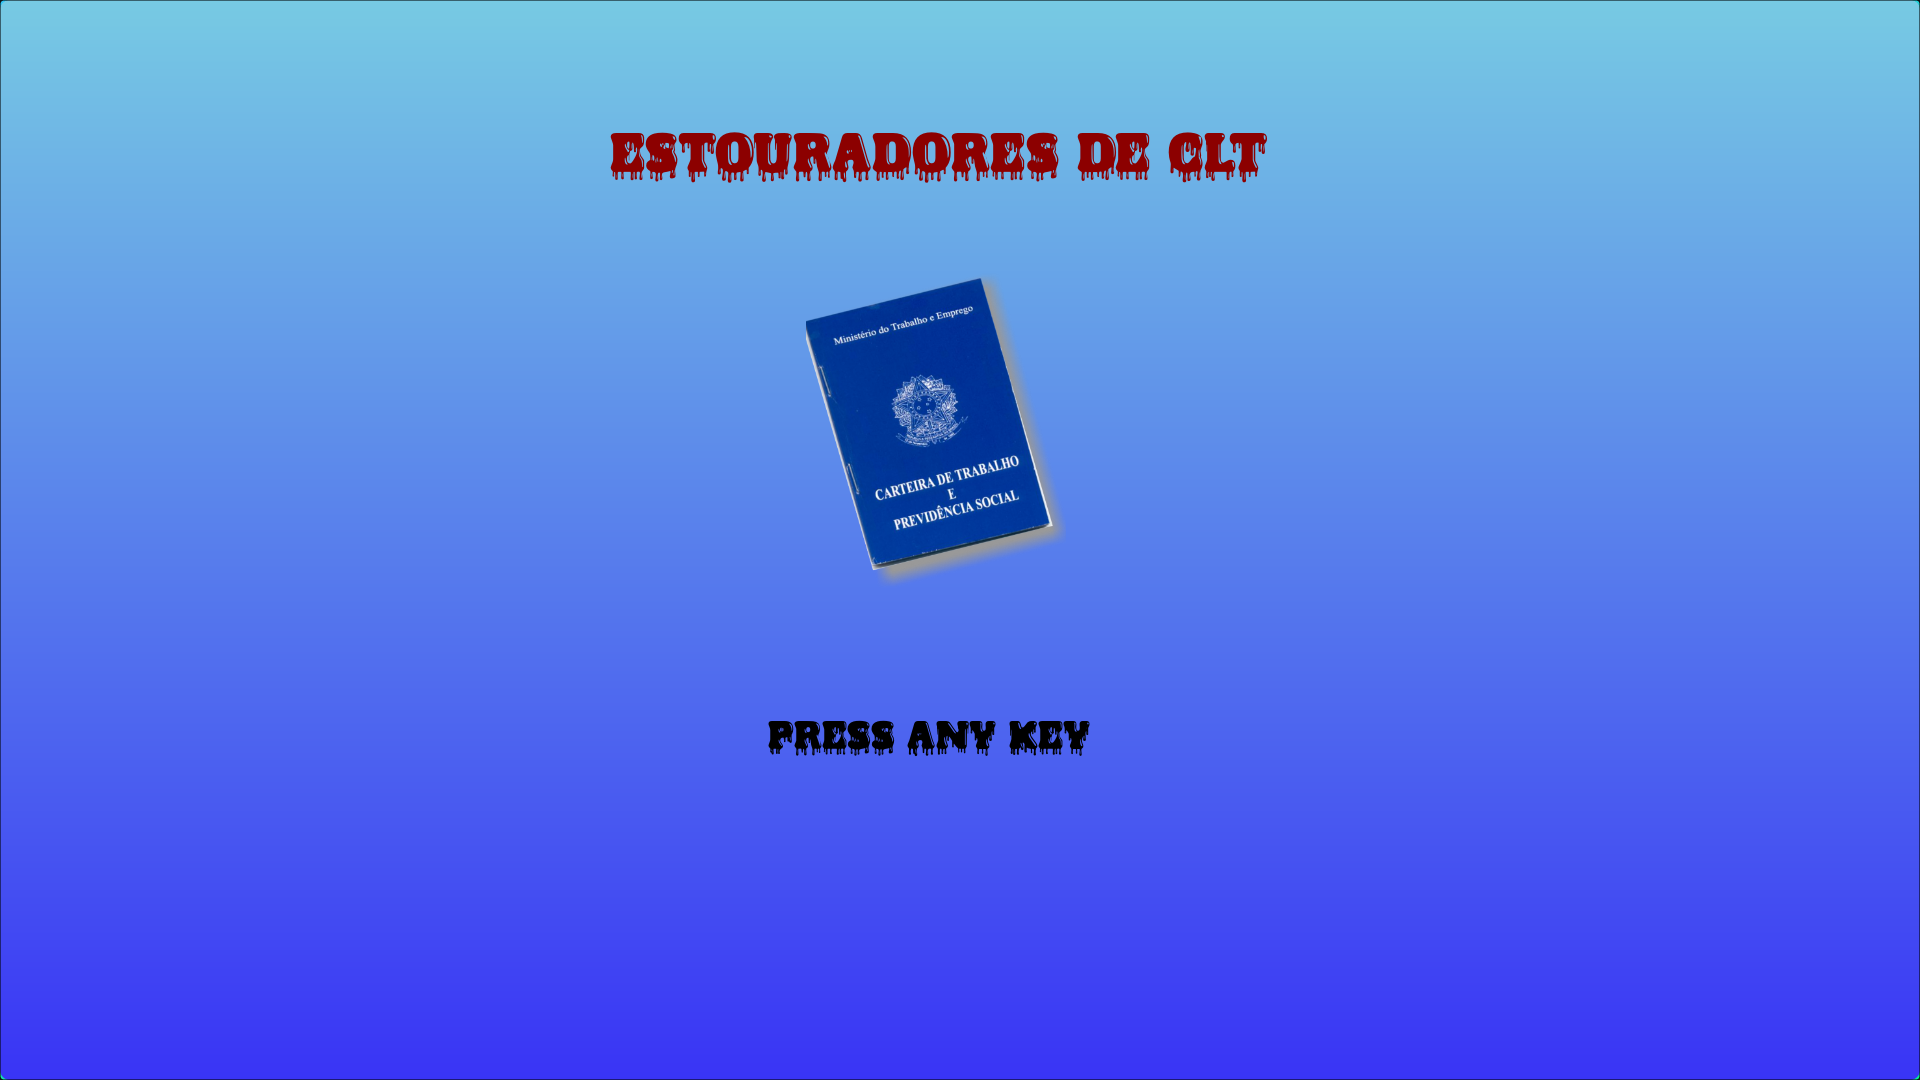
\includegraphics[width=0.9\textwidth]{imgs/inicio.png}
\caption{Menu Inicial}
\label{imagem 0.9}
\end{figure}
\begin{figure}[H]
\centering
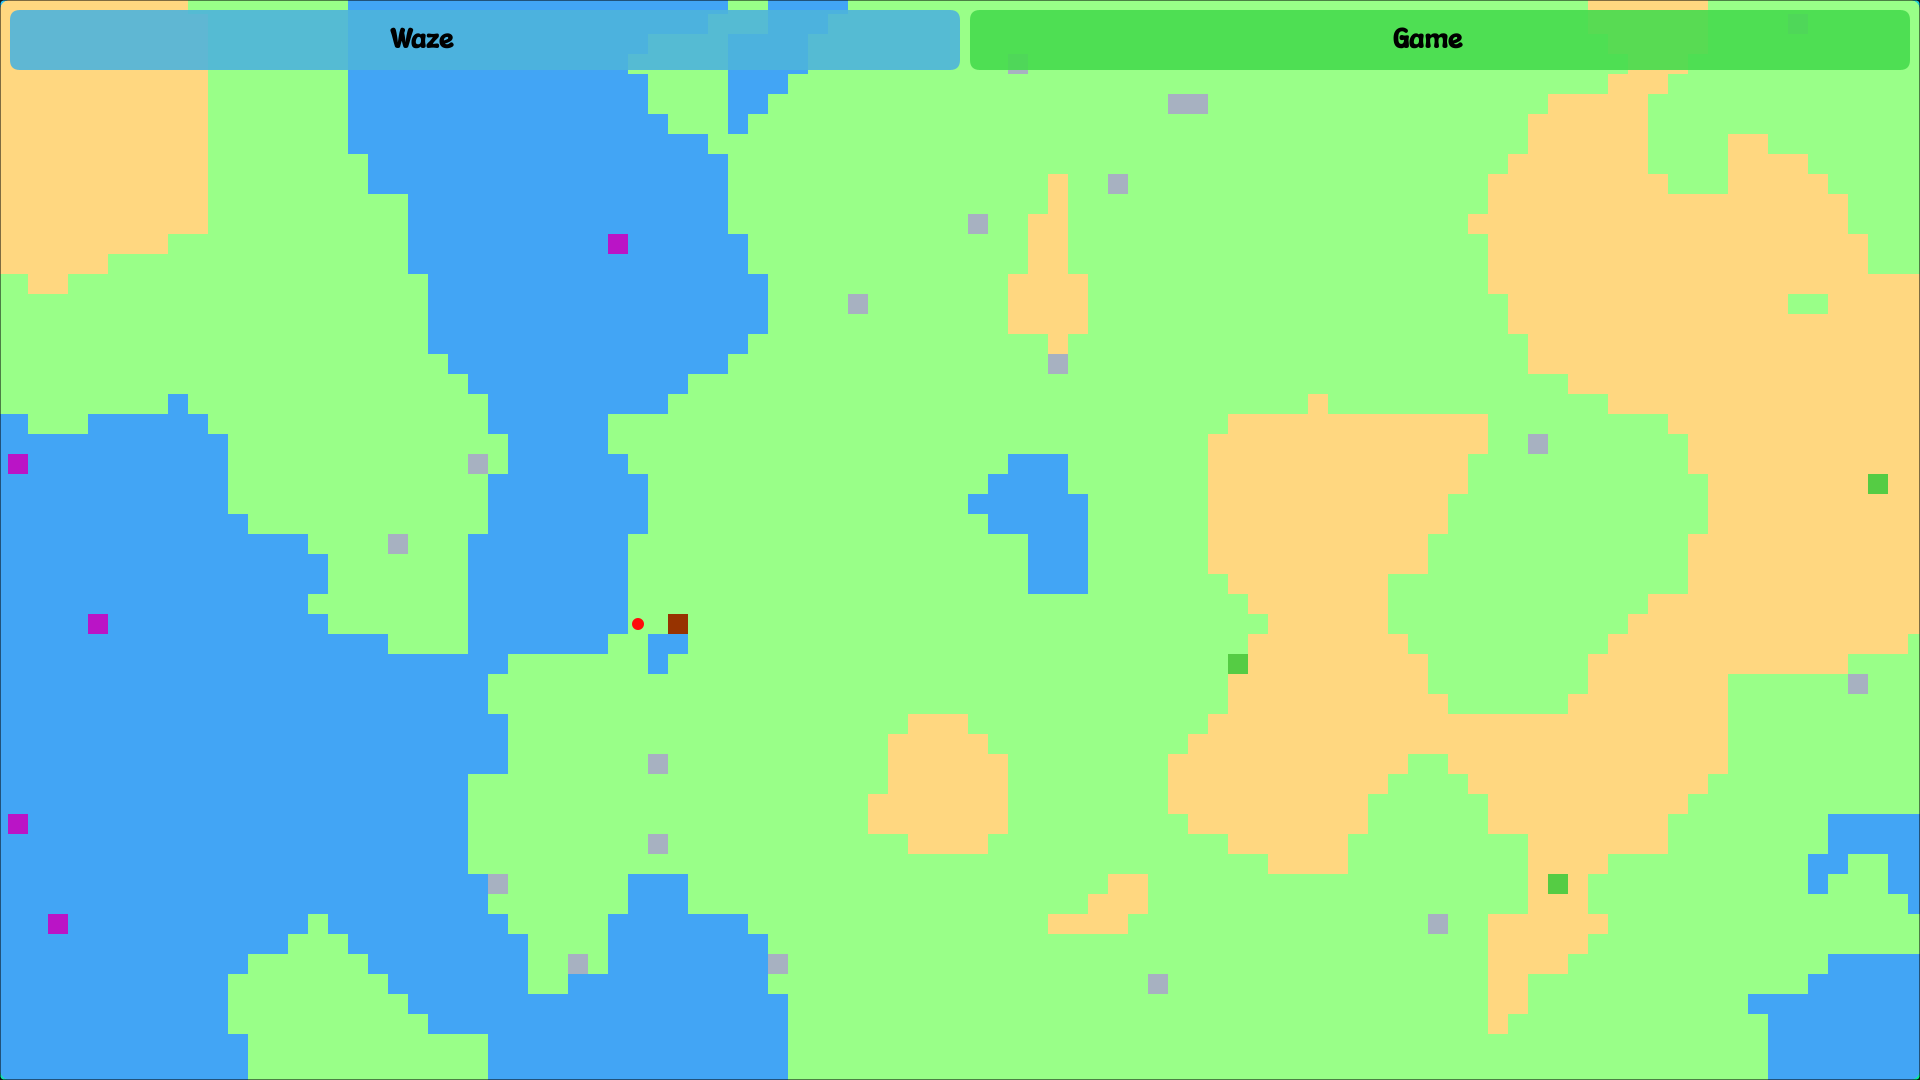
\includegraphics[width=0.9\textwidth]{imgs/agua.png}
\caption{Player impossibilitado de passar na água por não estar com barco (posicionado a sua direita)}
\label{imagem 5}
\end{figure}
\begin{figure}[H]
\centering
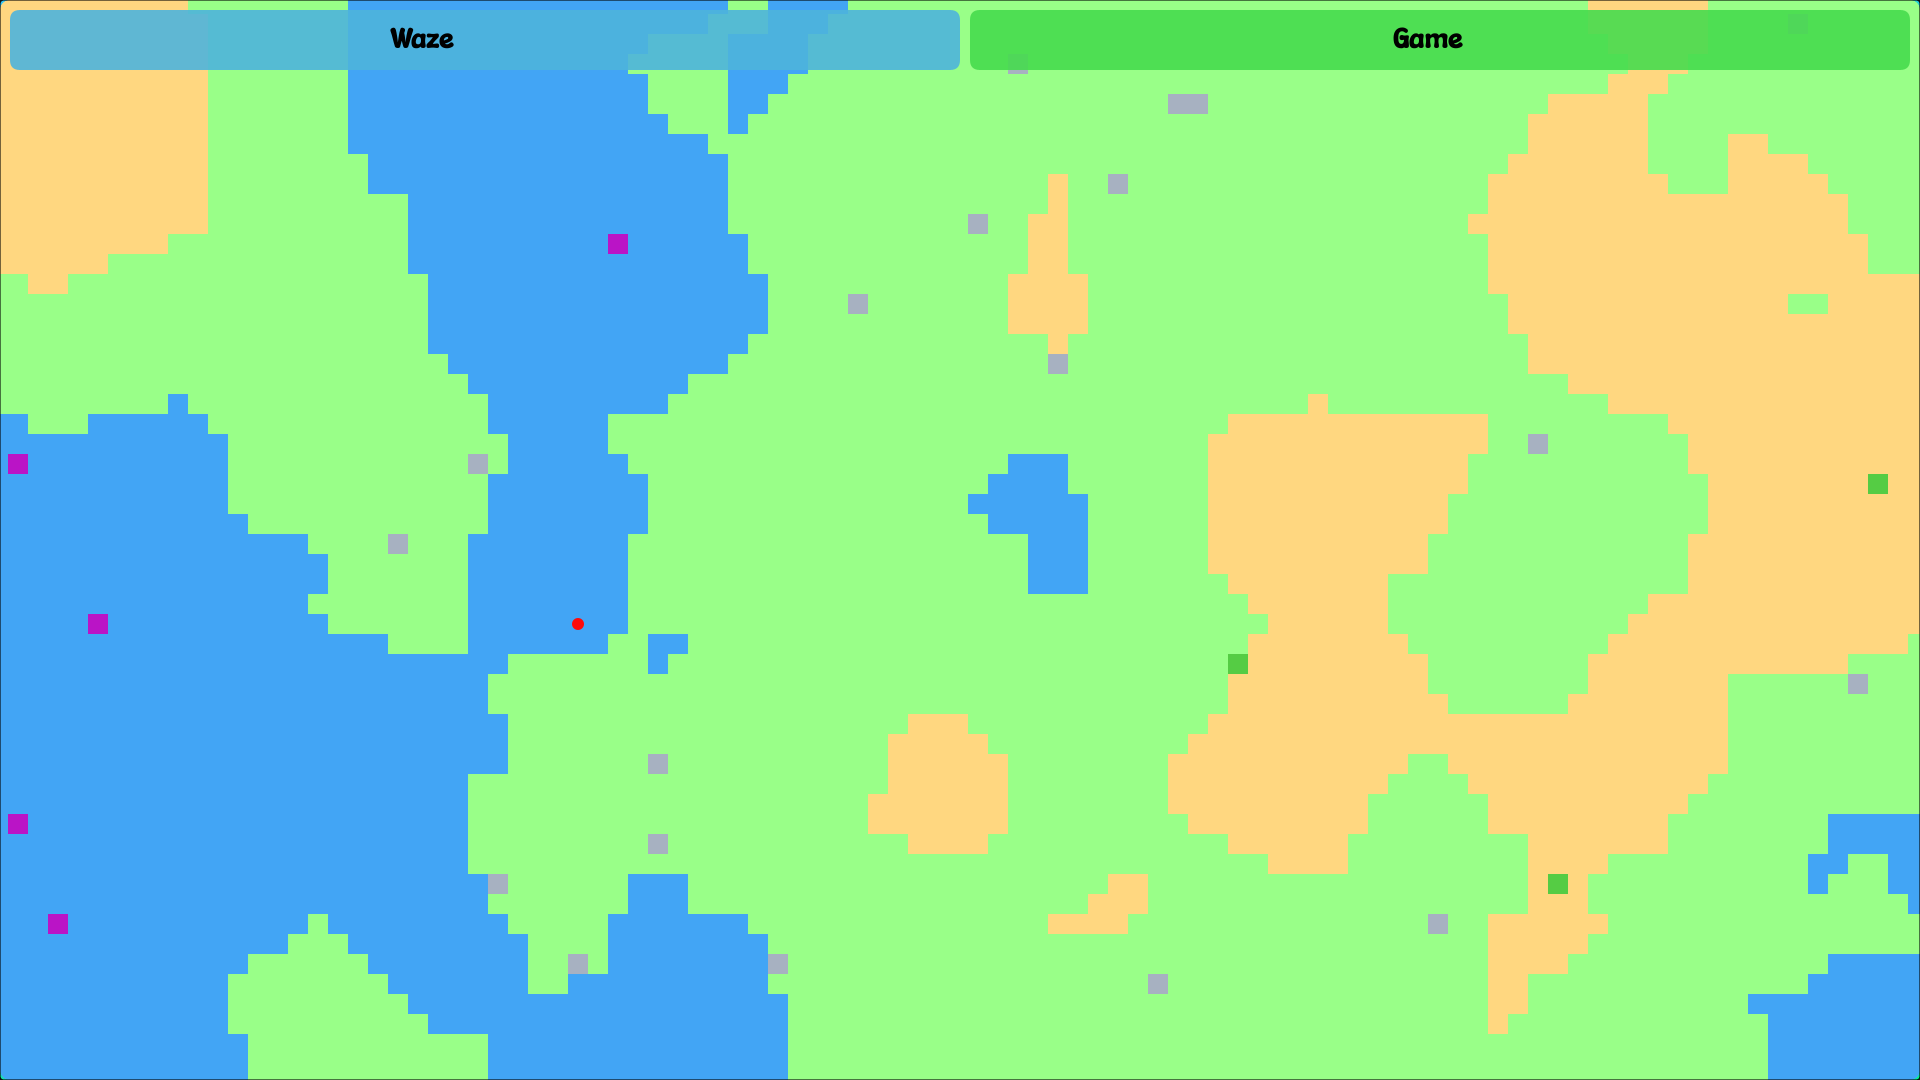
\includegraphics[width=0.9\textwidth]{imgs/agua-barco.png}
\caption{Player com barco na água}
\label{imagem 5}
\end{figure}
\begin{figure}[H]
\centering
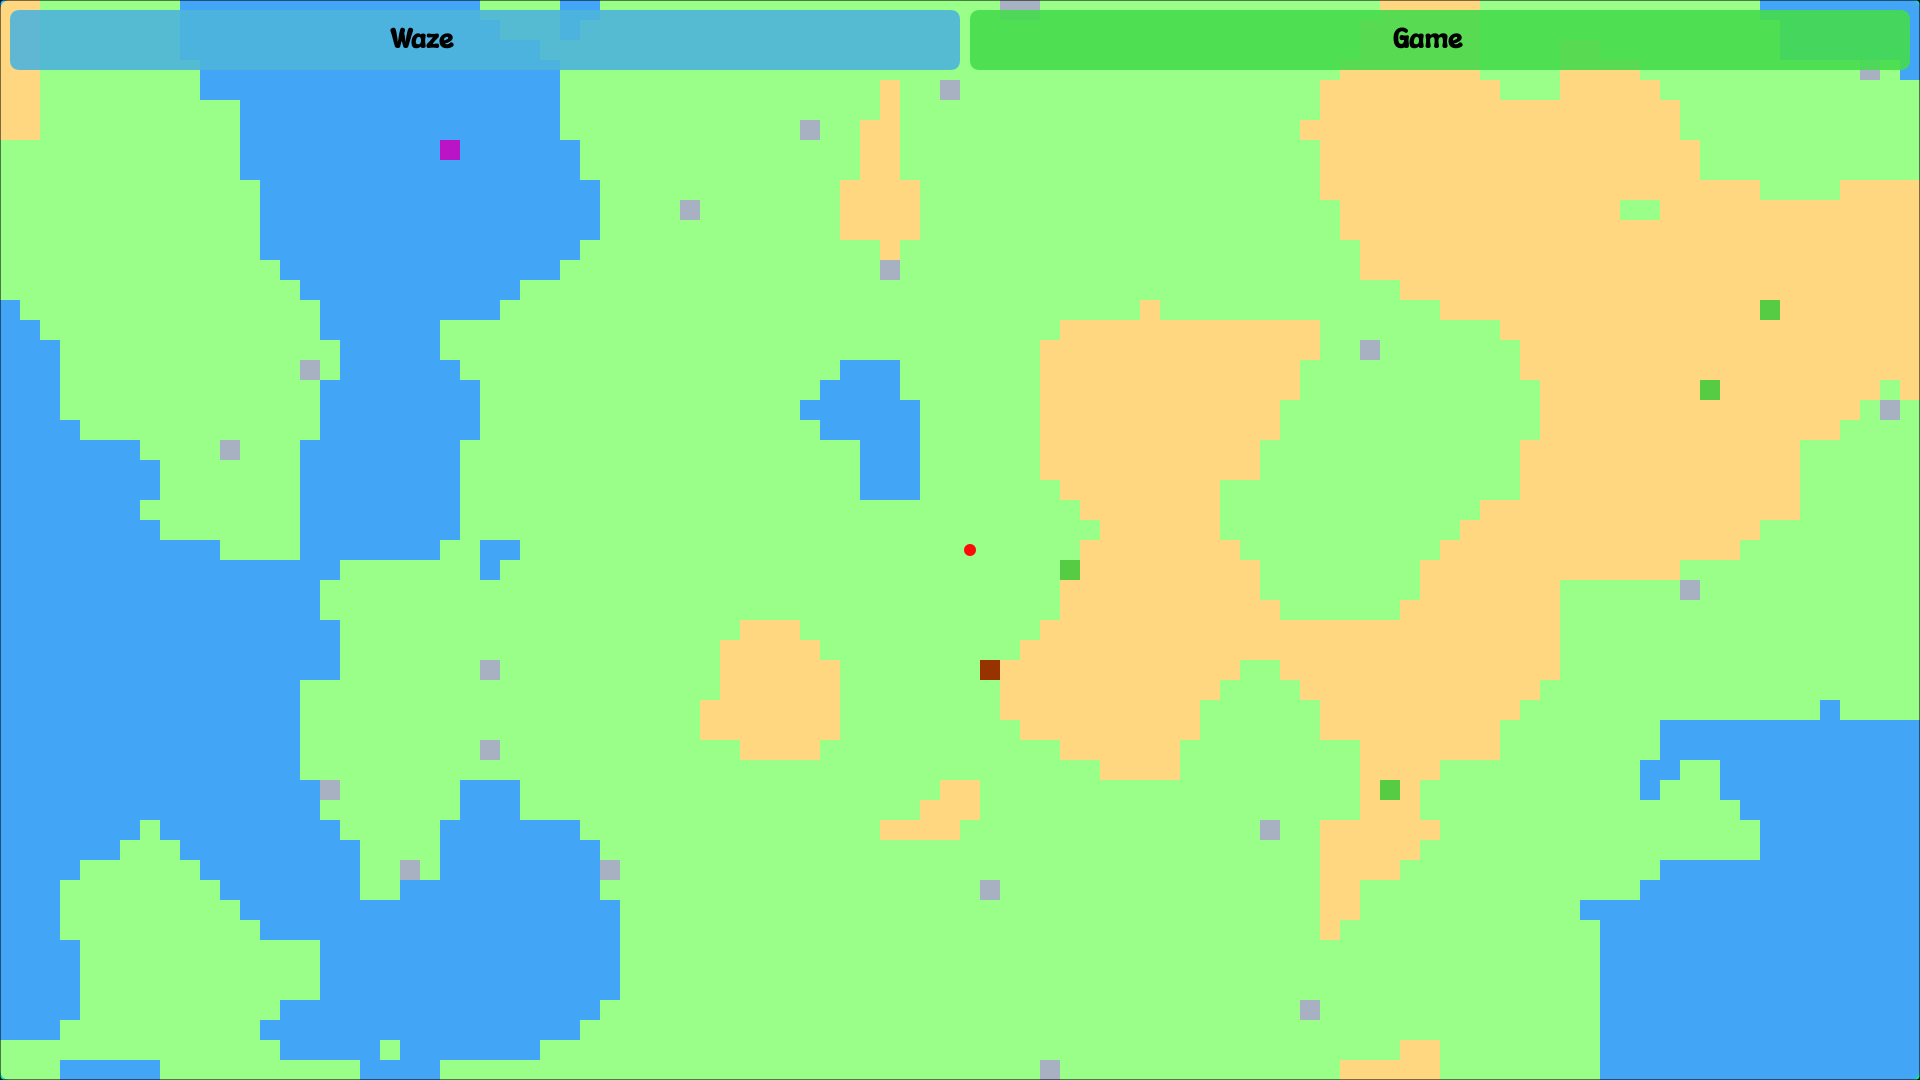
\includegraphics[width=0.9\textwidth]{imgs/escolha.png}
\caption{Menu de escolha entre os modos de jogo}
\label{imagem 5}
\end{figure}
\begin{figure}[H]
\centering
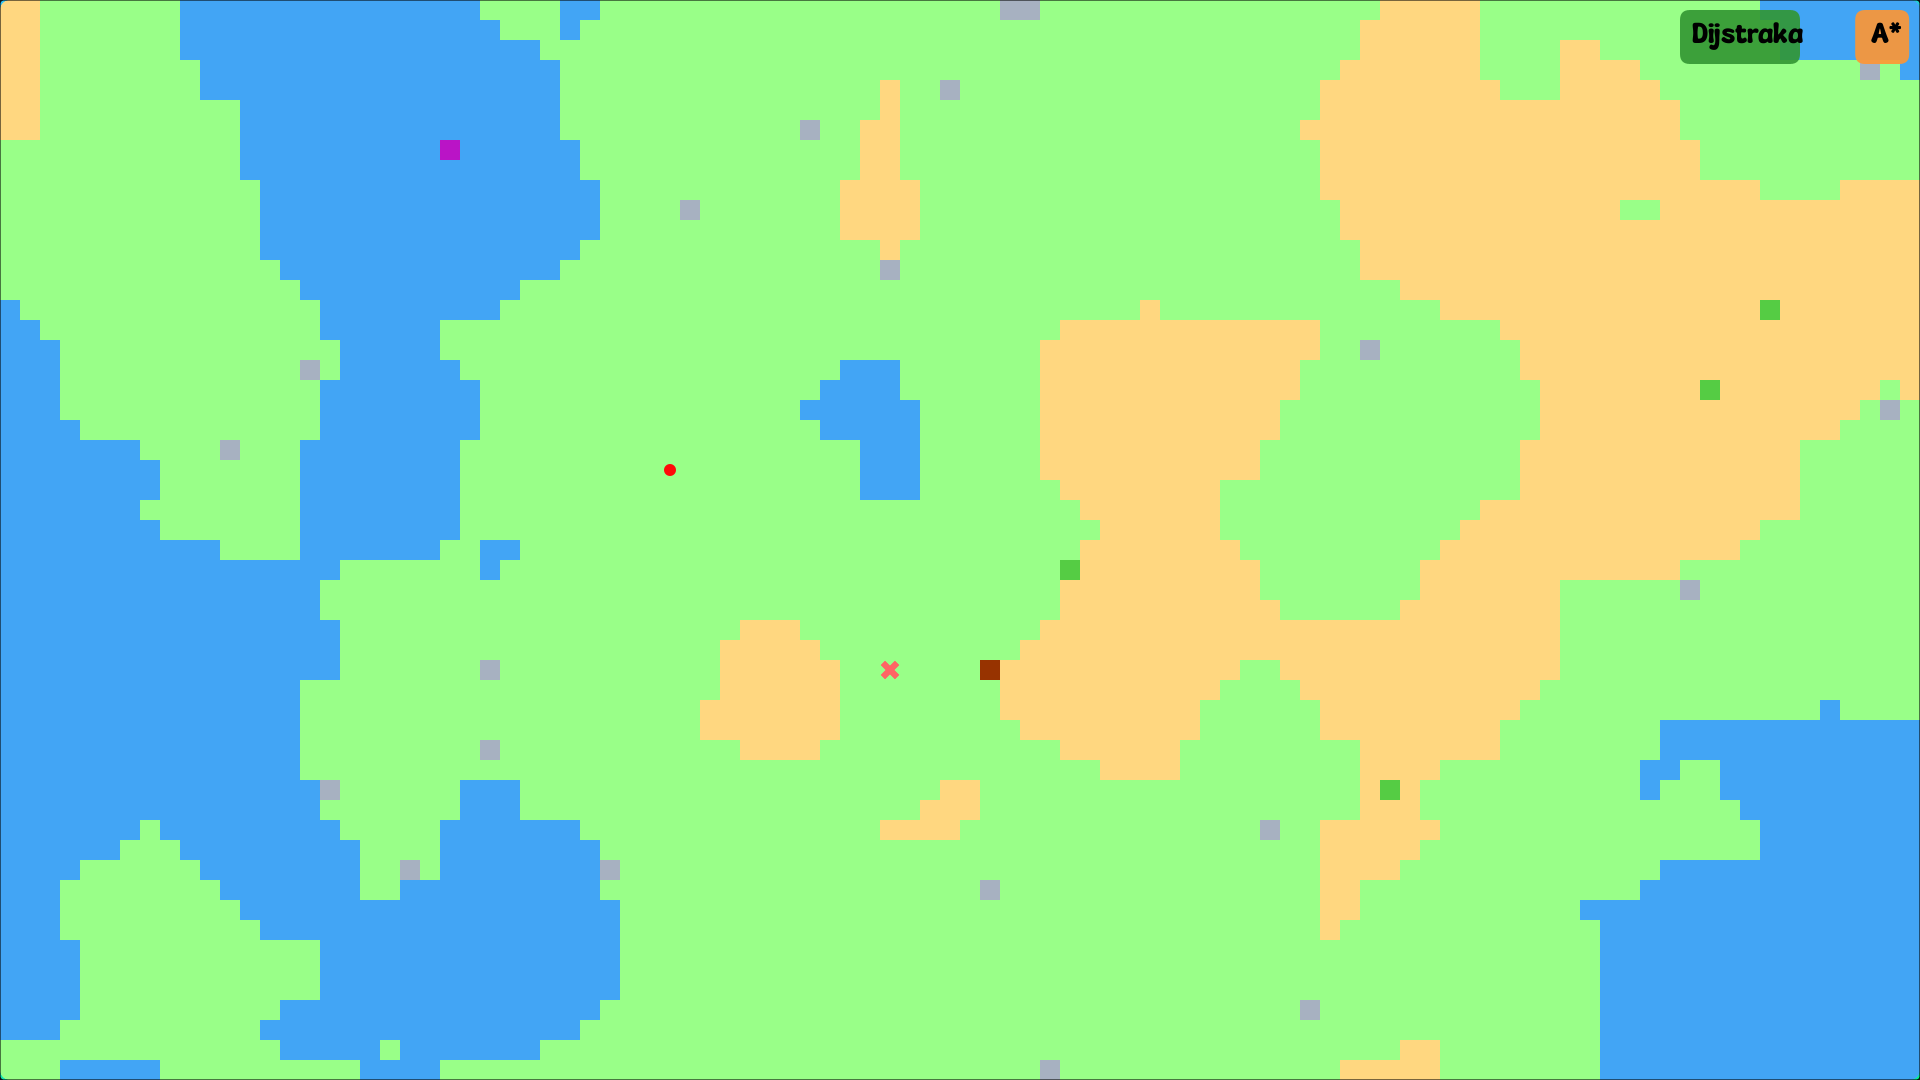
\includegraphics[width=0.9\textwidth]{imgs/waze-escolha.png}
\caption{Escolha de algoritmo no Waze}
\label{imagem 5}
\end{figure}
\begin{figure}[H]
\centering
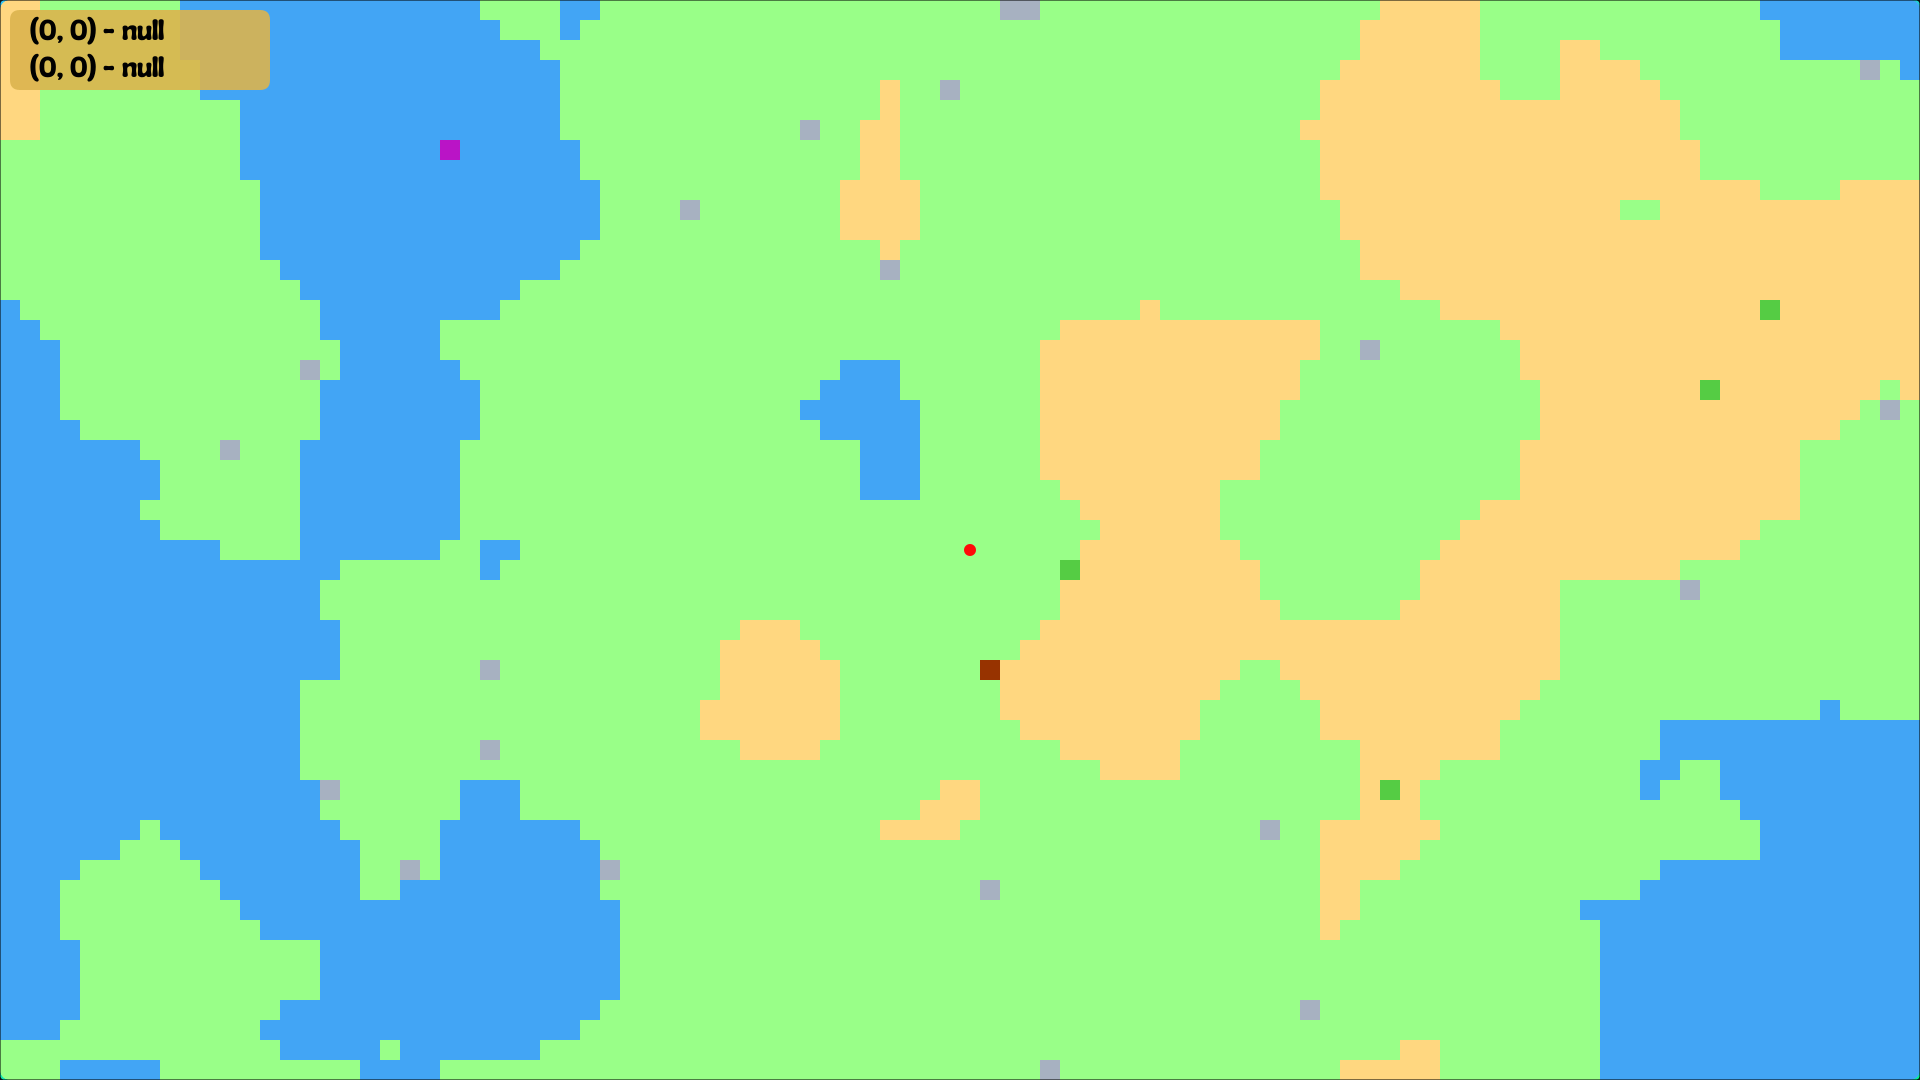
\includegraphics[width=0.9\textwidth]{imgs/waze-1.png}
\caption{Waze início}
\label{imagem 5}
\end{figure}
\begin{figure}[H]
\centering
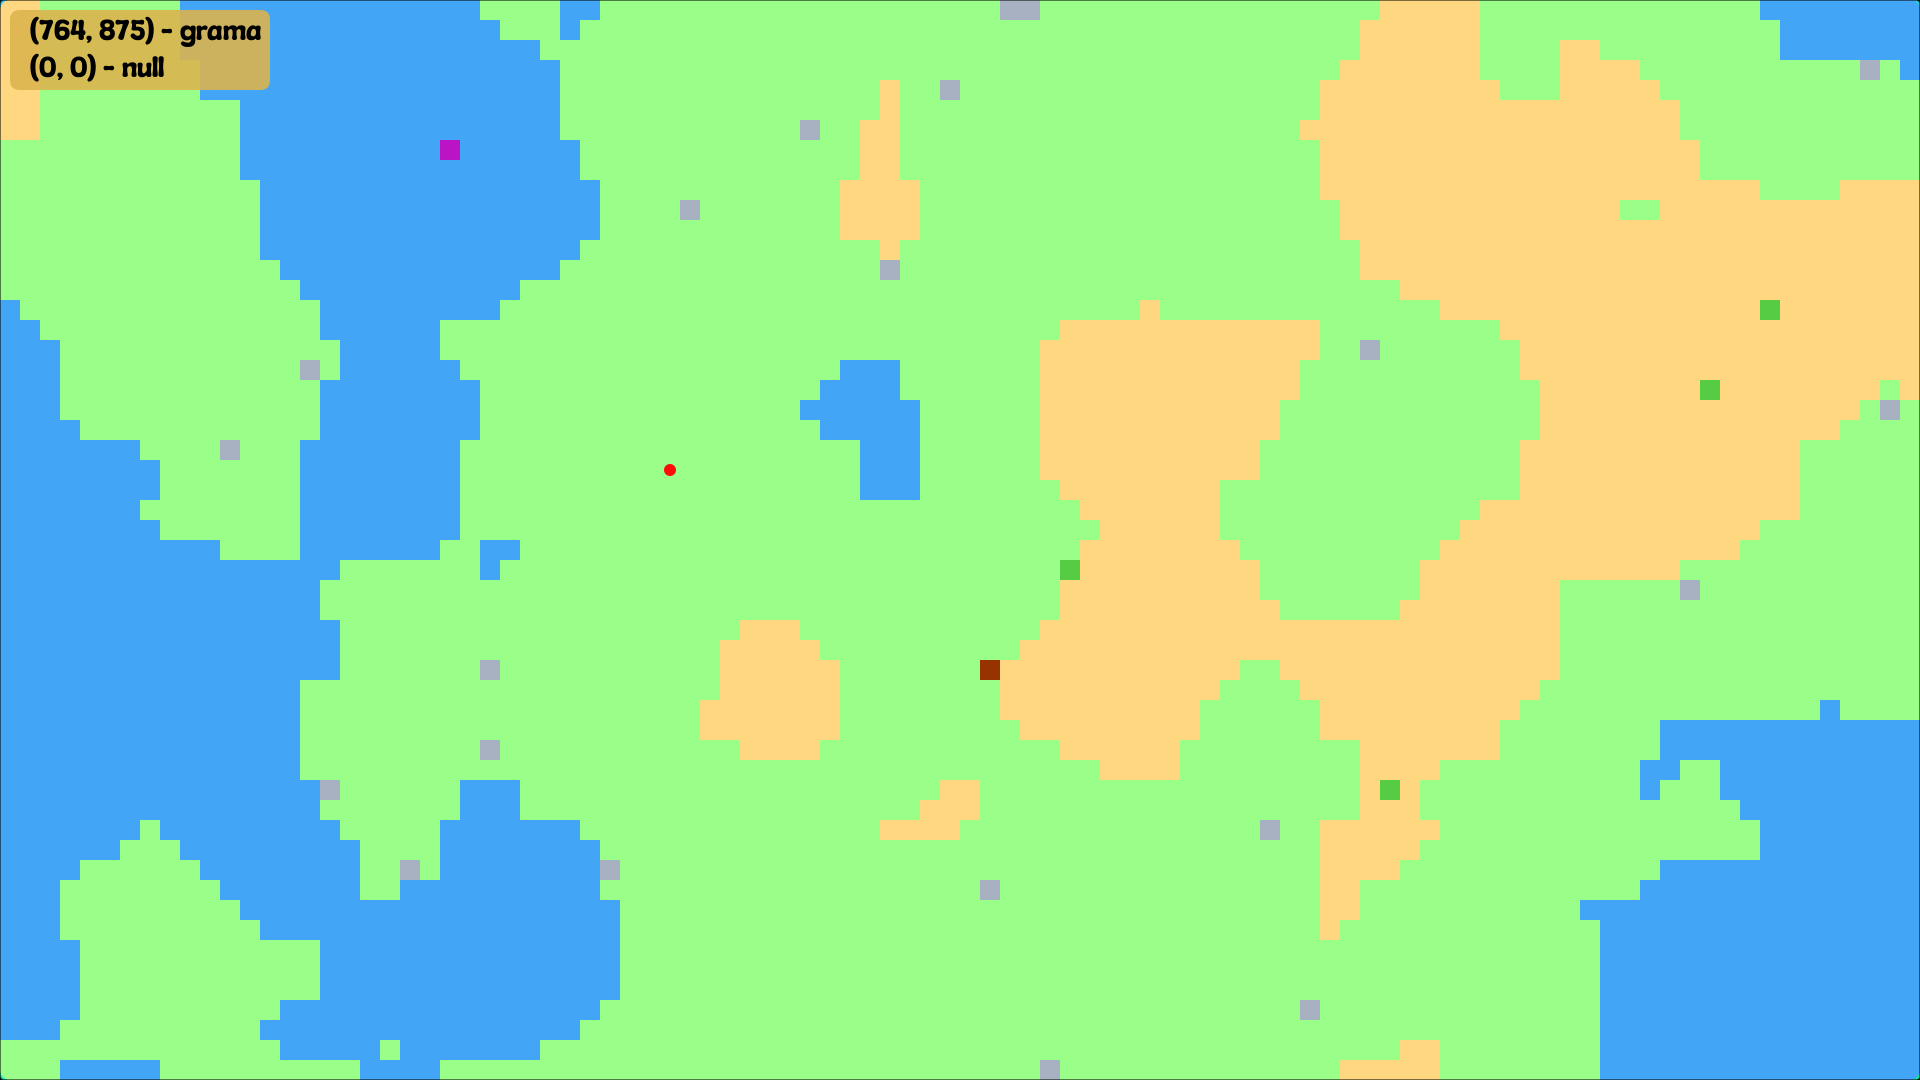
\includegraphics[width=0.9\textwidth]{imgs/waze-2.png}
\caption{Waze com origem selecionada}
\label{imagem 5}
\end{figure}
\begin{figure}[H]
\centering
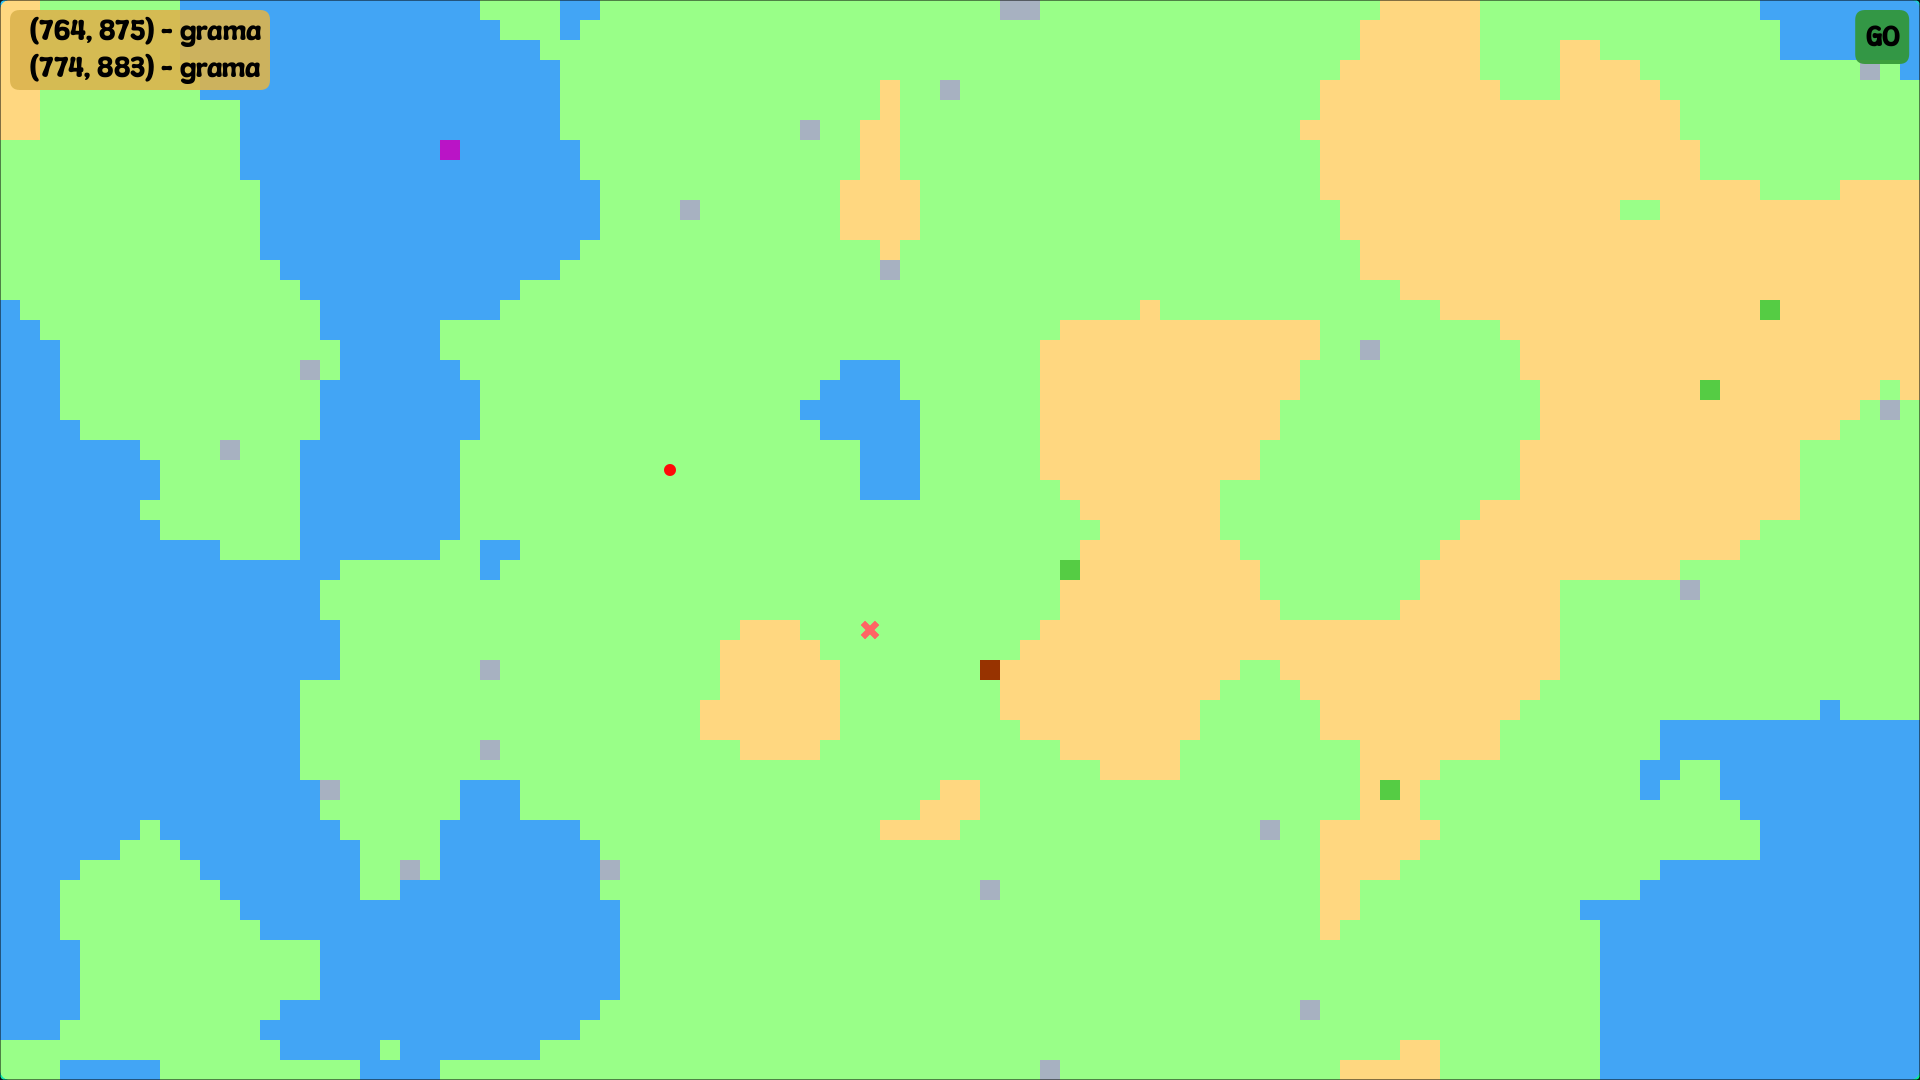
\includegraphics[width=0.9\textwidth]{imgs/waze-3.png}
\caption{Waze com destino selecionado}
\label{imagem 5}
\end{figure}
\begin{figure}[H]
\centering
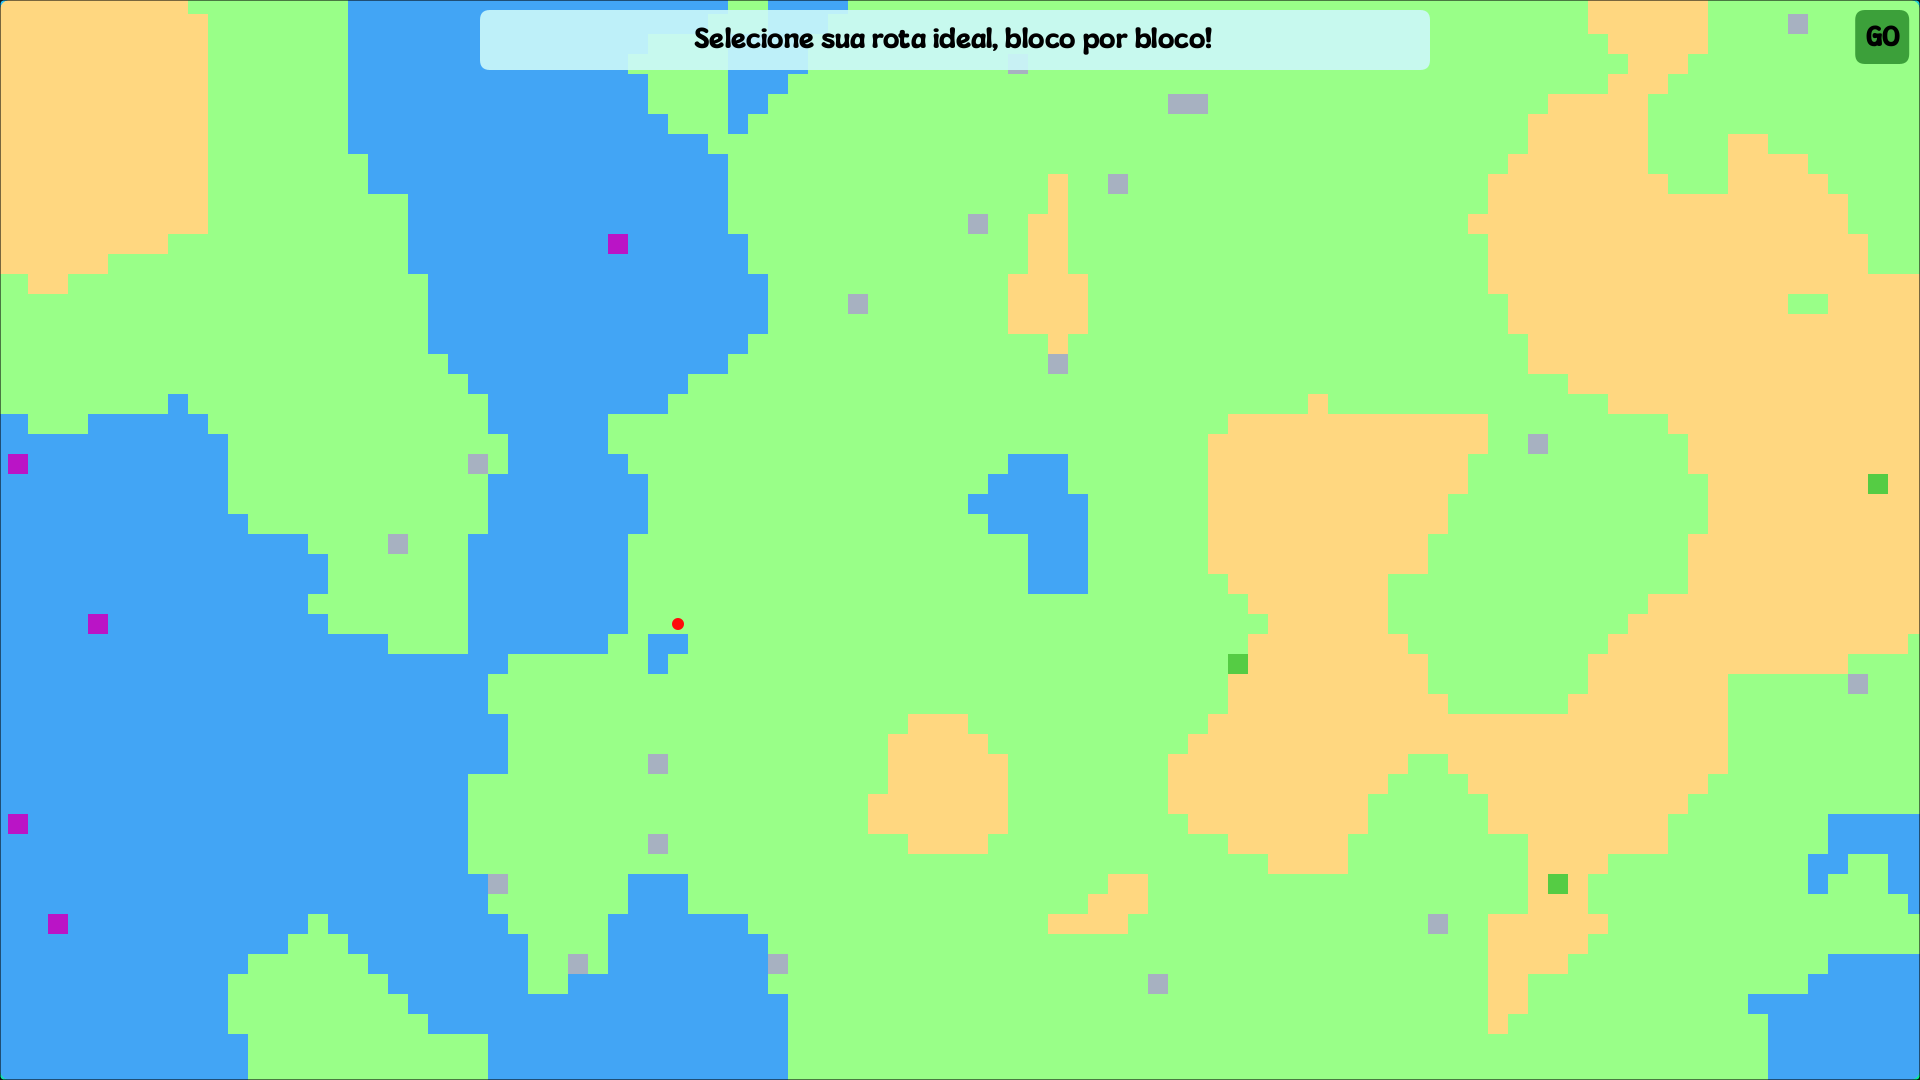
\includegraphics[width=0.9\textwidth]{imgs/pre-game-1.png}
\caption{Pré-game}
\label{imagem 3}
\end{figure}
\begin{figure}[H]
\centering
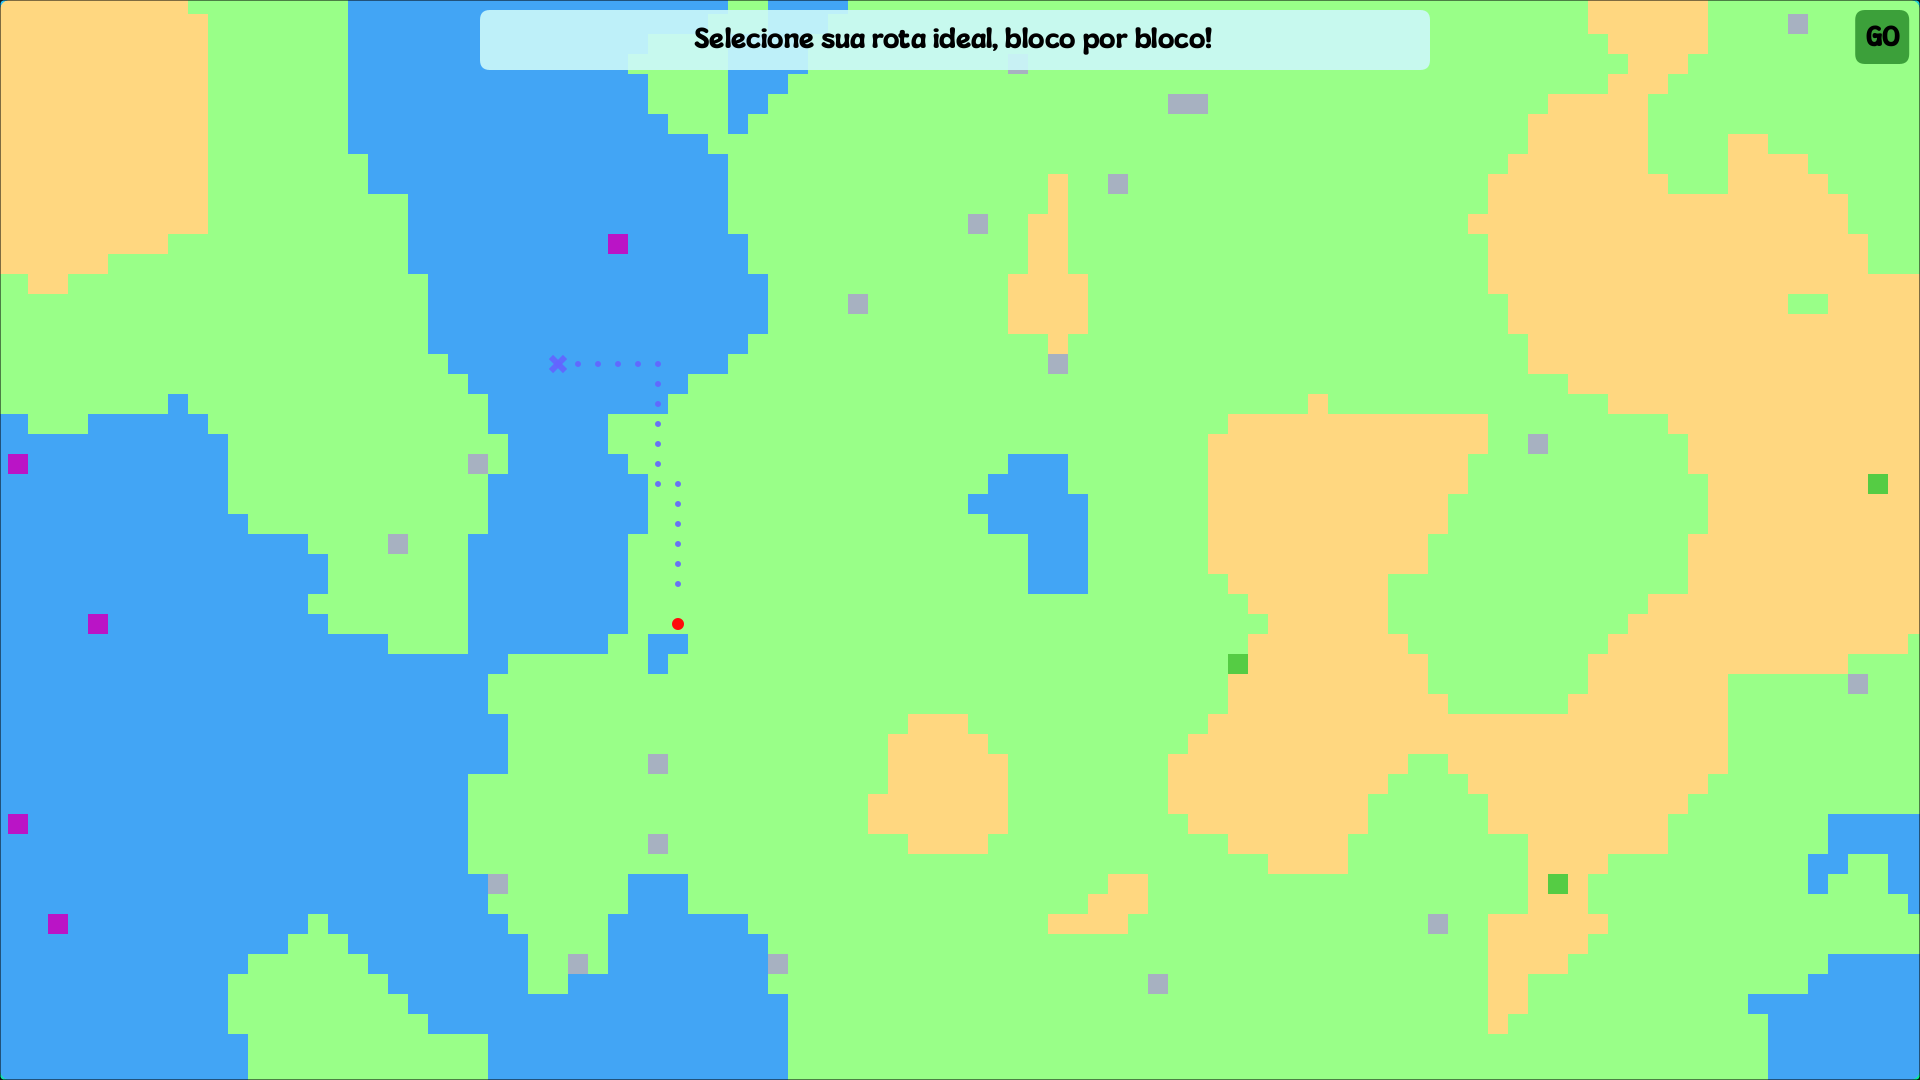
\includegraphics[width=0.9\textwidth]{imgs/pre-game-2.png}
\caption{Game com rota selecionada}
\label{imagem 4}
\end{figure}
\begin{figure}[H]
\centering
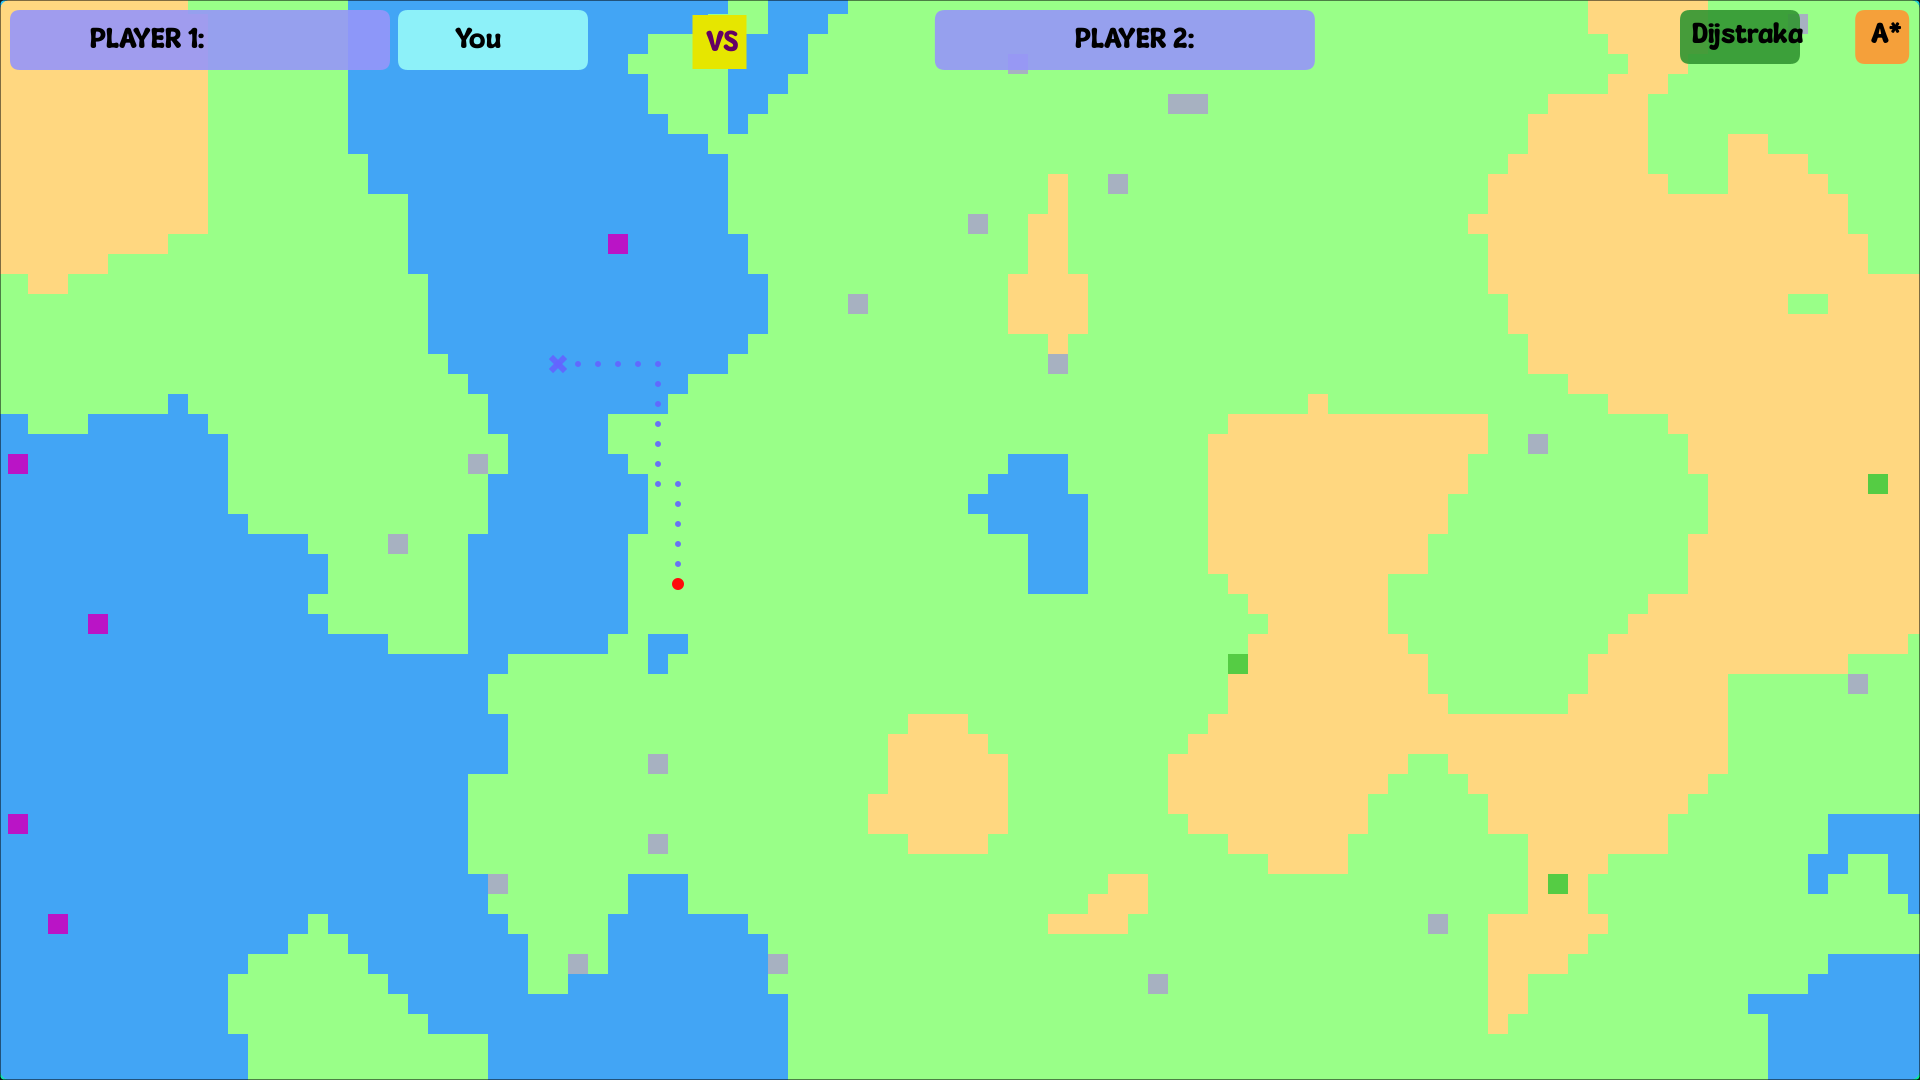
\includegraphics[width=0.9\textwidth]{imgs/inicio-game.png}
\caption{Tela de início Game}
\label{imagem 5}
\end{figure}
\begin{figure}[H]
\centering
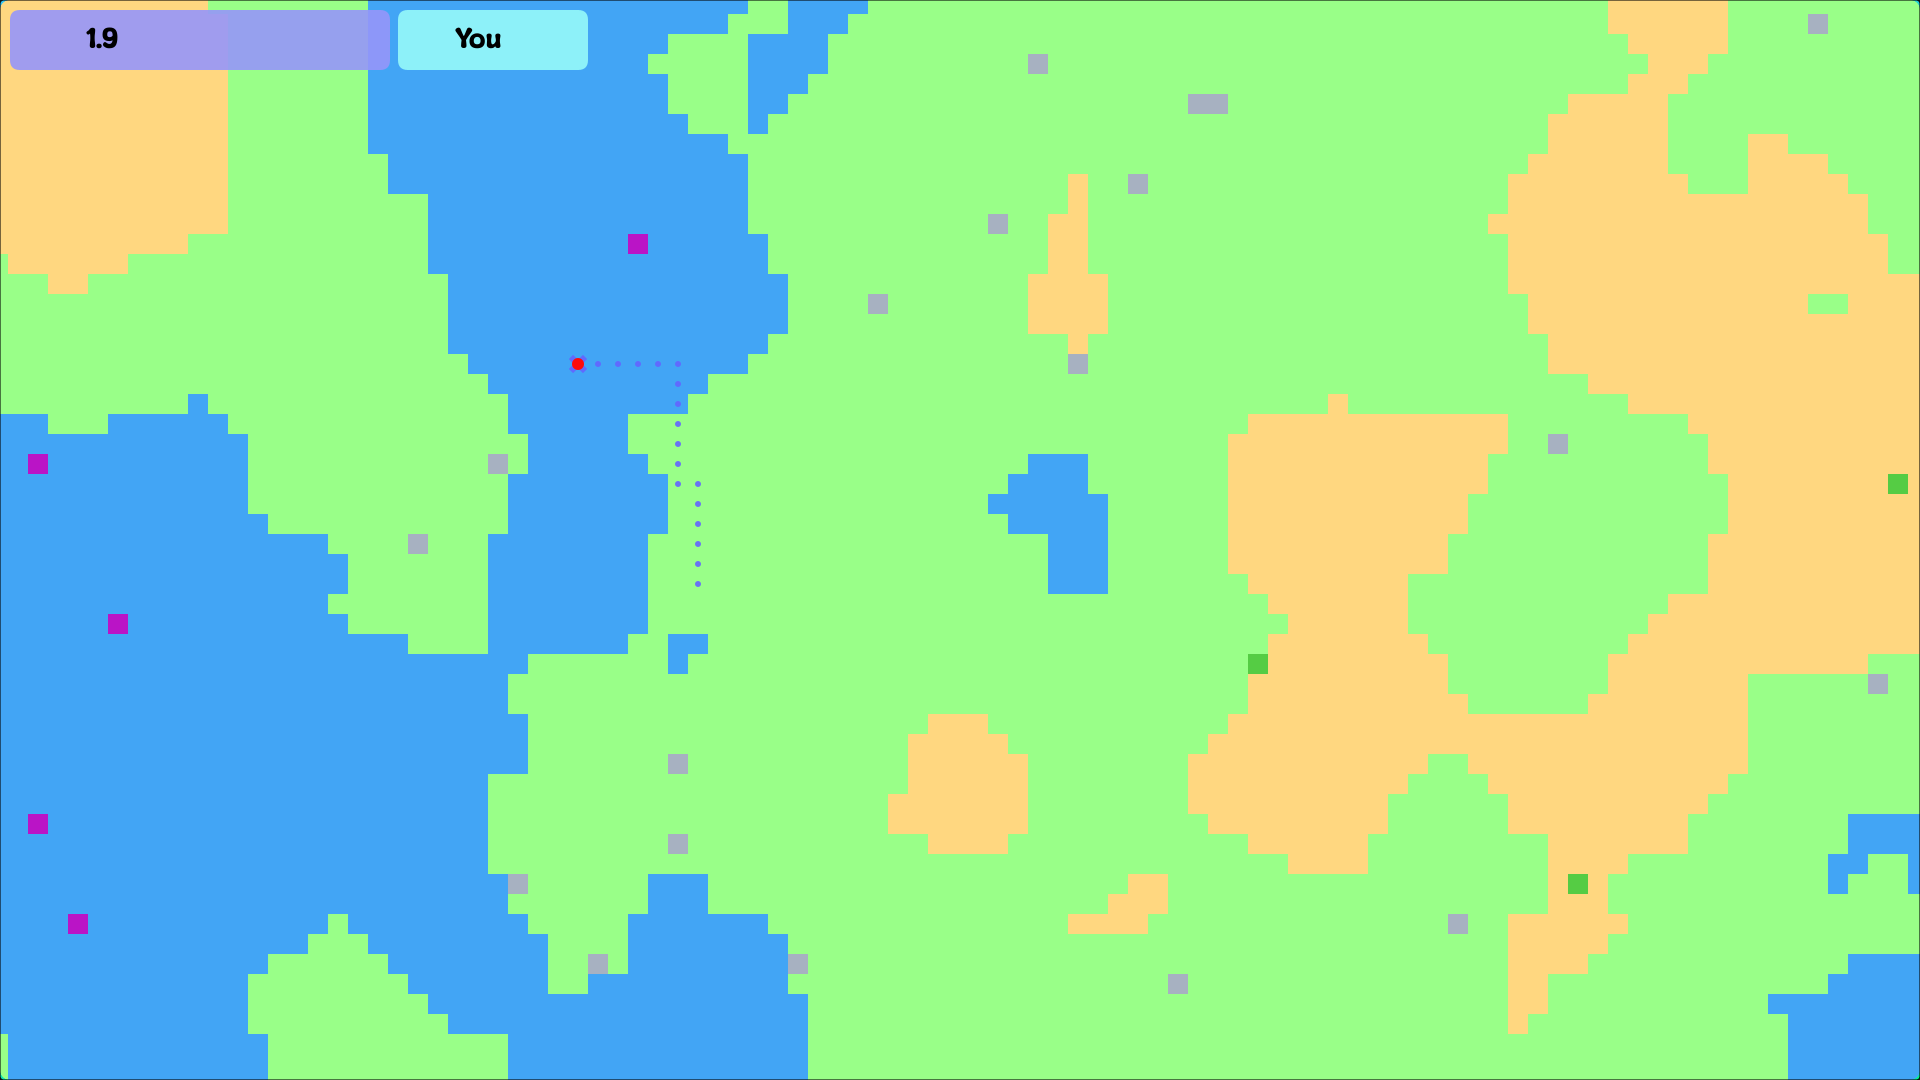
\includegraphics[width=0.9\textwidth]{imgs/player.png}
\caption{Game: Vez do Player}
\label{imagem 5}
\end{figure}
\begin{figure}[H]
\centering
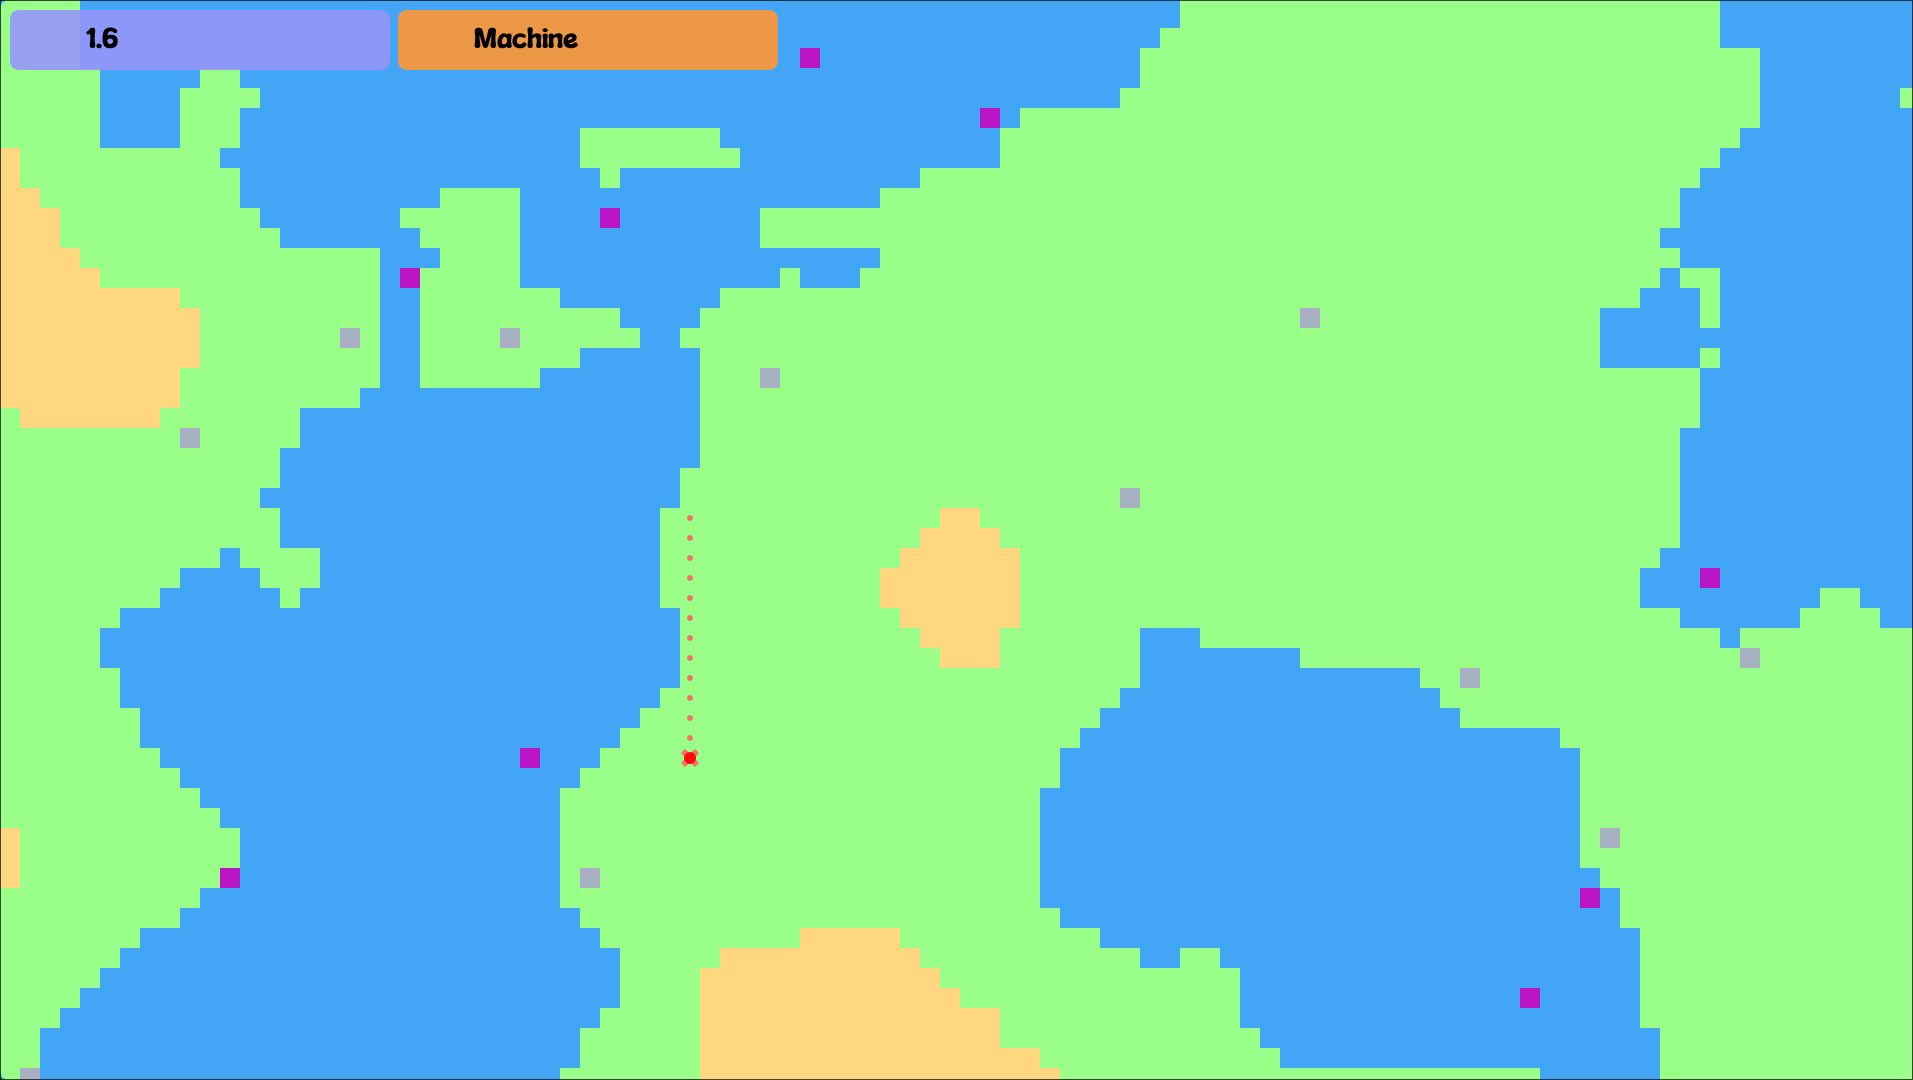
\includegraphics[width=0.9\textwidth]{imgs/machine.png}
\caption{Game: Vez do algortimo escolhido}
\label{imagem 5}
\end{figure}
\begin{figure}[H]
\centering
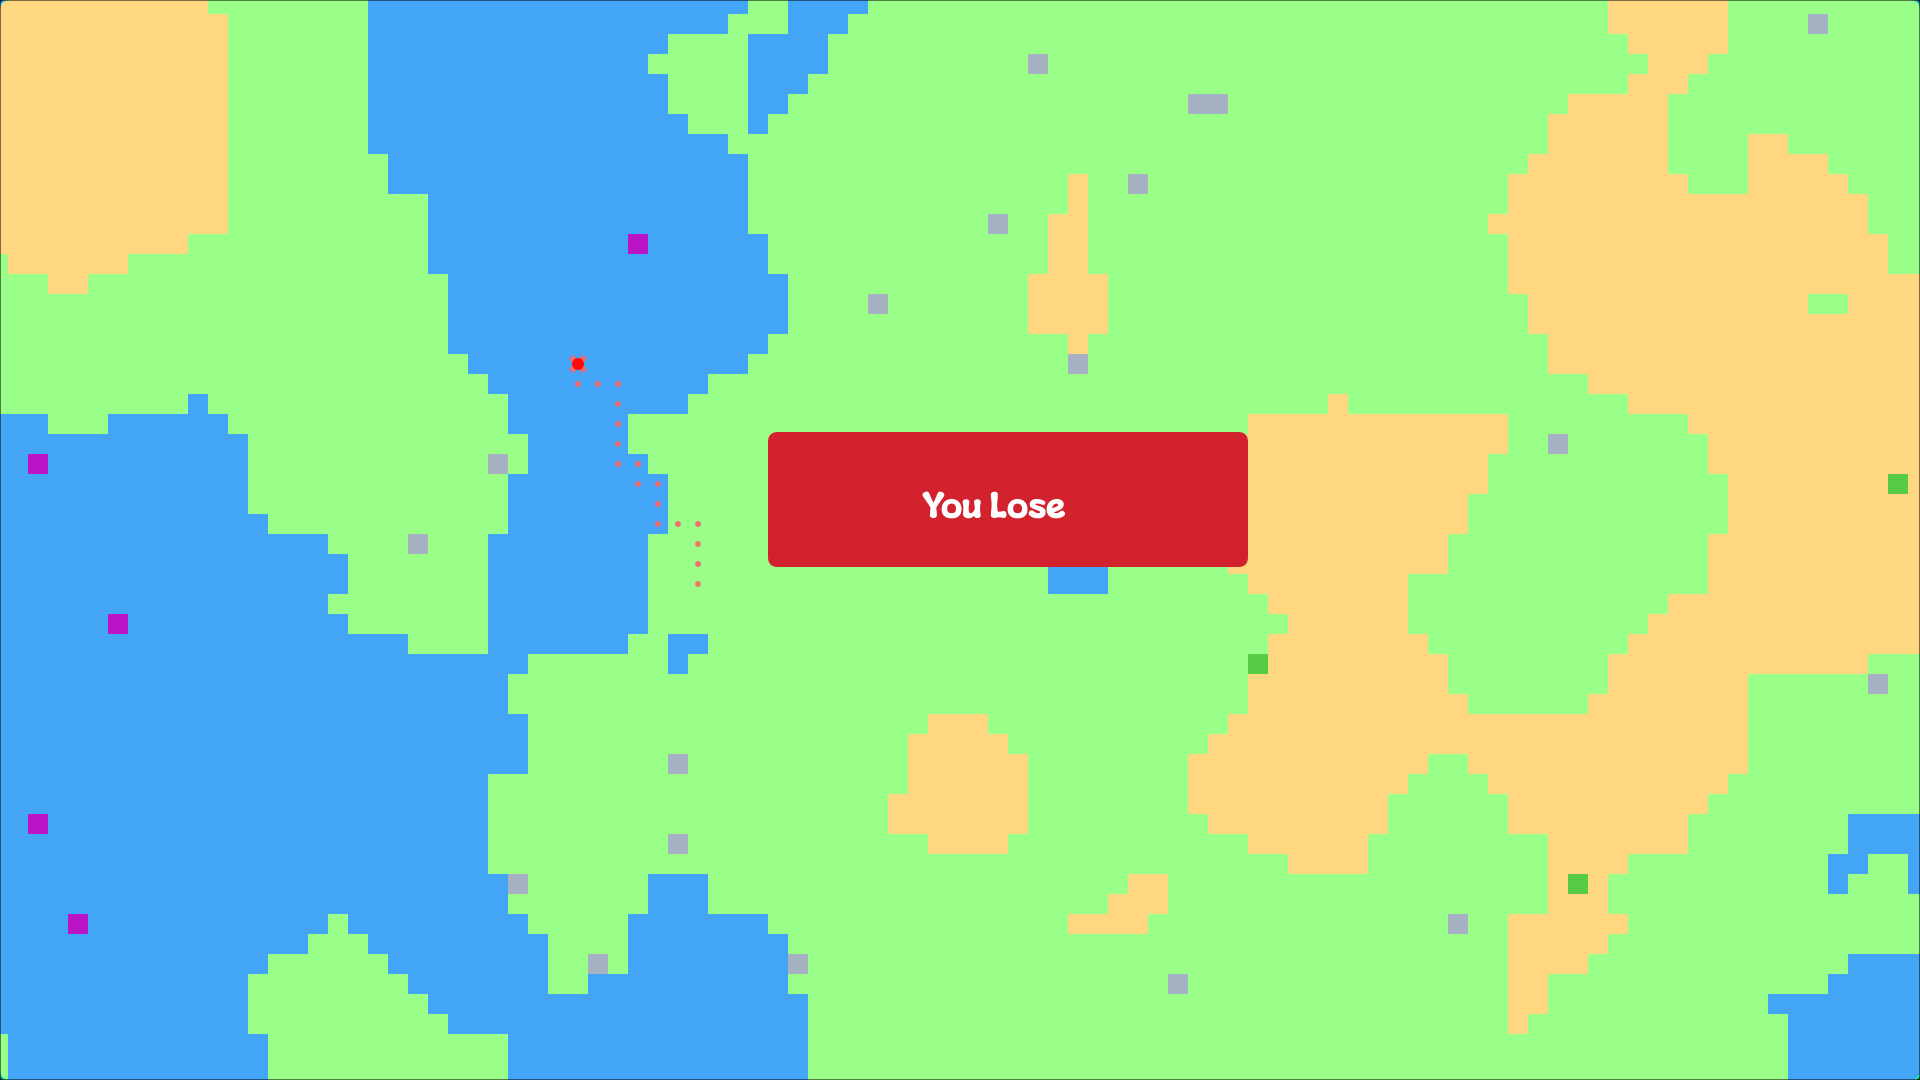
\includegraphics[width=0.9\textwidth]{imgs/derrota.png}
\caption{Game: Derrota}
\label{imagem 5}
\end{figure}
\begin{figure}[H]
\centering
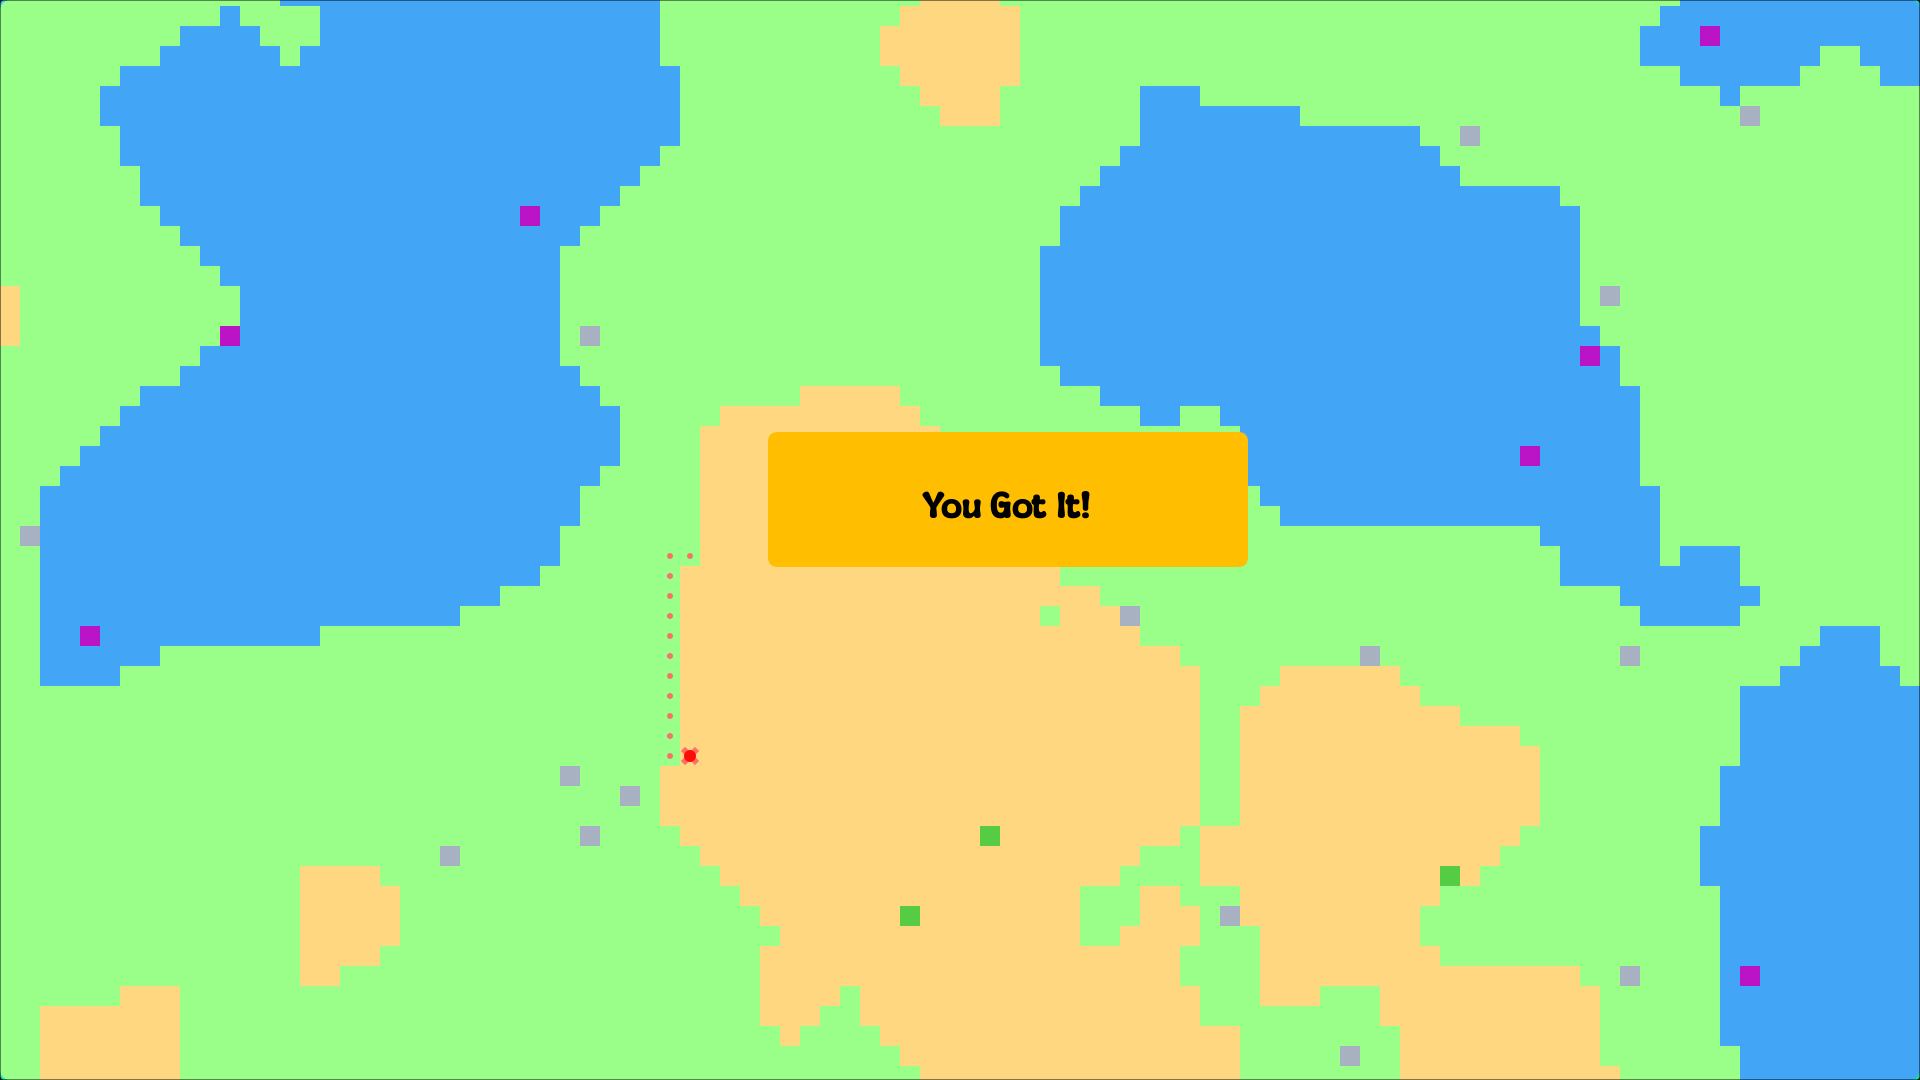
\includegraphics[width=0.9\textwidth]{imgs/empate.png}
\caption{Game: Empate}
\label{imagem 5}
\end{figure}
\begin{figure}[H]
\centering
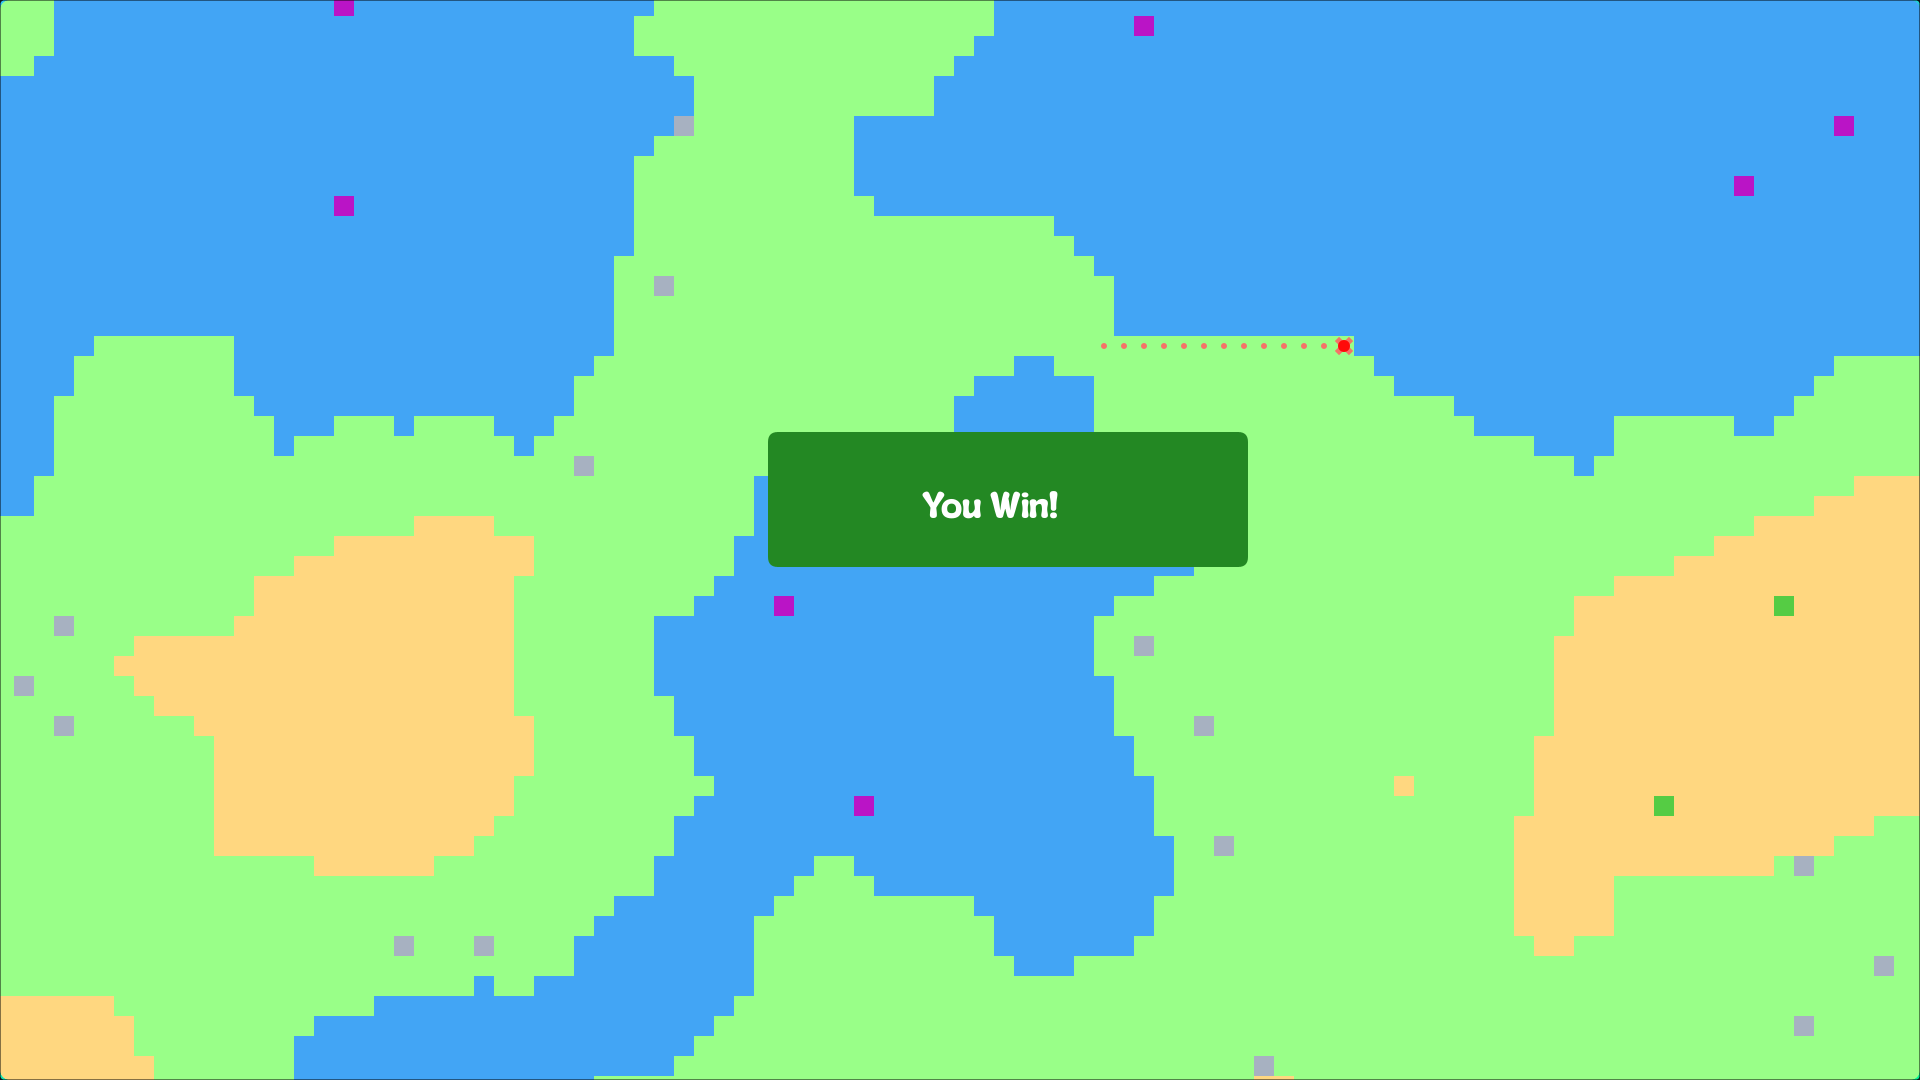
\includegraphics[width=0.9\textwidth]{imgs/vitoria.png}
\caption{Game: Vitória}
\label{imagem 5}
\end{figure}

Vale a pena observar que a vitória só ocorre quando é selecionada um rota em que a origem e o destino estão na mesma linha, mas é mais veloz se deslocar usando os blocos que não estão nessa linha. Nesse caso, só é fornecido o retângulo do vértice origem ao destino, não sendo vistos os blocos mais vantajosos fora dele.

\section{Conclusão}

O presente relatório apresentou a implementação de um jogo que simula um ambiente de navegação em um mapa com diferentes tipos de terreno e obstáculos. O jogo foi desenvolvido utilizando a linguagem de programação Java e a biblioteca Processing.

A implementação do jogo incluiu a criação de uma classe Map que gerencia o mapa e os chunks, uma classe Chunk que representa uma parte do terreno, uma classe Player que controla o movimento do jogador, uma classe Route que calcula o caminho mais curto entre dois pontos e uma classe Game que gerencia o fluxo do jogo.

O jogo foi testado e apresentou resultados satisfatórios, com a capacidade de gerar mapas aleatórios, calcular caminhos mais curtos e simular o movimento do jogador.

\subsection{Principais contribuições}

Implementação de um jogo que simula um ambiente de navegação em um mapa com diferentes tipos de terreno e obstáculos.
Criação de uma classe Map que gerencia o mapa e os chunks.
Criação de uma classe Chunk que representa uma parte do terreno.
Criação de uma classe Player que controla o movimento do jogador.
Criação de uma classe Route que calcula o caminho mais curto entre dois pontos.
Criação de uma classe Game que gerencia o fluxo do jogo.

\subsection{Limites e sugestões para possíveis melhorias}
A implementação do jogo pode ser melhorada com a adição de mais recursos, como a capacidade de salvar e carregar jogos.
A classe Map pode ser melhorada com a adição de mais tipos de terreno e obstáculos.
A classe Chunk pode ser melhorada com a adição de mais detalhes, como a capacidade de gerar terrenos mais complexos.
A classe Player pode ser melhorada com a adição de mais recursos, como a capacidade de saltar ou usar itens.
A classe Route pode ser melhorada com a melhora da feature que faz o algoritmo só testar as possibilidade dentro do retângulo criado do vértice origem ao destino, fazendo ele testar pontos um poucos mais amplos para possibilitar que o menor caminho seja sempre alcançado.
\subsection{Conclusão final}

O presente relatório apresentou a implementação de um jogo que simula um ambiente de navegação em um mapa com diferentes tipos de terreno e obstáculos, mais o uso de algoritmos de menor caminho, fazendo os presentes autores se aprofundarem na implementação prática, mais ligada ao mundo real, desses algoritmos. A implementação do jogo foi satisfatória e apresentou resultados positivos. No entanto, há espaço para melhorias e sugestões para futuras melhorias foram apresentadas.

\end{document}
